\section{Điểm,đường thẳng,mặt phẳng trong không gian}

\subsection{Đề 1}
\Opensolutionfile{ans}[ans/ans-0-B1]
\caulc

\begin{ex}%[1H4H1-3]-Câu 1
	Trong mặt phẳng $\left(\alpha\right)$, cho tứ giác $ ABCD$ có $ AB$ cắt $ CD$ tại $ E$, $ AC$ cắt $ BD$ tại $ F$, $ S$ là điểm không thuộc $\left(\alpha\right)$. Giao tuyến của $\left(SAB\right)$và $\left(SCD\right)$ là
	\choice
	{$ SF$}
	{$SD$}
	{$ AC$}
	{\True $ SE$}
	\loigiai{
		\begin{center}
			
			
			\tikzset{every picture/.style={line width=0.75pt}} %set default line width to 0.75pt        
			
			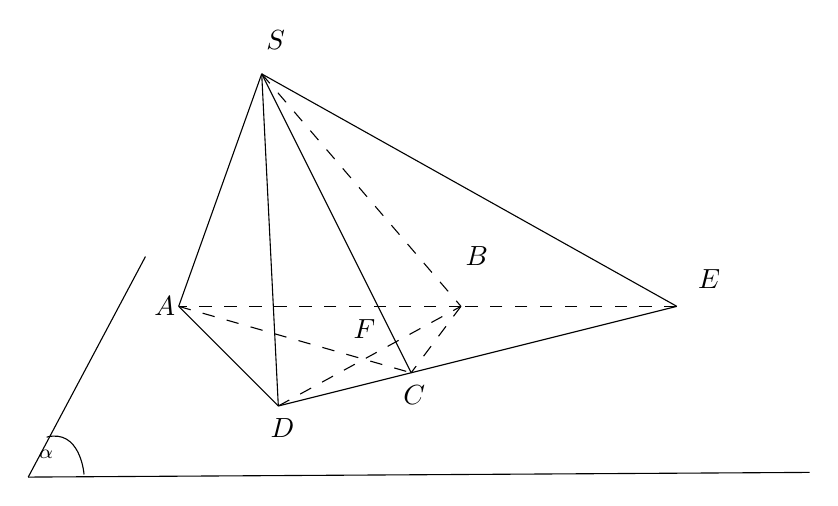
\begin{tikzpicture}[x=0.75pt,y=0.75pt,yscale=-1,xscale=1]
				%uncomment if require: \path (0,300); %set diagram left start at 0, and has height of 300
				
				%Straight Lines [id:da8055441080935524] 
				\draw    (143.51,234.26) -- (520,232) ;
				%Straight Lines [id:da44371795807755565] 
				\draw    (200,128) -- (143.51,234.26) ;
				%Curve Lines [id:da2633492196274172] 
				\draw    (152.38,215) .. controls (168.38,211) and (170.38,232) .. (170.38,233) ;
				%Straight Lines [id:da8022641909188839] 
				\draw  [dash pattern={on 4.5pt off 4.5pt}]  (352,152) -- (216,152) ;
				%Straight Lines [id:da7429557683362615] 
				\draw    (216,152) -- (264,200) ;
				%Straight Lines [id:da6448687935452875] 
				\draw    (328,184) -- (264,200) ;
				%Straight Lines [id:da9701343779587384] 
				\draw  [dash pattern={on 4.5pt off 4.5pt}]  (352,152) -- (328,184) ;
				%Straight Lines [id:da48224499197435255] 
				\draw    (456,152) -- (328,184) ;
				%Straight Lines [id:da7422907840707798] 
				\draw  [dash pattern={on 4.5pt off 4.5pt}]  (456,152) -- (352,152) ;
				%Straight Lines [id:da38807285296002836] 
				\draw    (256,40) -- (216,152) ;
				%Straight Lines [id:da4192647605232809] 
				\draw    (256,40) -- (264,200) ;
				%Straight Lines [id:da799980725193379] 
				\draw    (256,40) -- (328,184) ;
				%Straight Lines [id:da6784673944015782] 
				\draw  [dash pattern={on 4.5pt off 4.5pt}]  (256,40) -- (352,152) ;
				%Straight Lines [id:da39080075305805306] 
				\draw    (256,40) -- (456,152) ;
				%Straight Lines [id:da1733812267288508] 
				\draw  [dash pattern={on 4.5pt off 4.5pt}]  (216,152) -- (328,184) ;
				%Straight Lines [id:da7976755810168057] 
				\draw  [dash pattern={on 4.5pt off 4.5pt}]  (264,200) -- (352,152) ;
				
				% Text Node
				\draw (147.38,220) node [anchor=north west][inner sep=0.75pt]  [font=\scriptsize] [align=left] {$\alpha$};
				% Text Node
				\draw (257,18) node [anchor=north west][inner sep=0.75pt]   [align=left] {$S$};
				% Text Node
				\draw (203,146) node [anchor=north west][inner sep=0.75pt]   [align=left] {$A$};
				% Text Node
				\draw (353,122) node [anchor=north west][inner sep=0.75pt]   [align=left] {$B$};
				% Text Node
				\draw (323,189) node [anchor=north west][inner sep=0.75pt]   [align=left] {$C$};
				% Text Node
				\draw (259,205) node [anchor=north west][inner sep=0.75pt]   [align=left] {$D$};
				% Text Node
				\draw (465,133) node [anchor=north west][inner sep=0.75pt]   [align=left] {$E$};
				% Text Node
				\draw (299,157) node [anchor=north west][inner sep=0.75pt]   [align=left] {$F$};
			\end{tikzpicture}
		\end{center}
		ta có $\heva{&S\in (SAB)\\&S\in (SCD)}$
		$\Rightarrow S$ là điểm chung thứ 1.\\
		$\heva{&E\in AB, AB\subset (SAB)\Rightarrow S\in (SAB)\\&E\in CD, CD\subset (SCD)\Rightarrow E\in (SCD)}\Rightarrow E$ là điểm chung thứ 2.\\
		Do đó $SE$ là giao tuyến của 2 mặt phẳng $SCD$ và $SAB$.\\
		}
\end{ex}

\begin{ex}%[1H4H1-3]-Câu 2
	Cho hình chóp $ S.ABCD$. Gọi $ O$ là giao điểm của $ AC$ và $ BD$. Giao tuyến của hai mặt phẳng $\left(SAC\right)$ và $\left(SBD\right)$ là đường thẳng
	\choice
	{$ SM$}
	{\True $ SO$}
	{$ SN$}
	{$ MN$}
	\loigiai{
		\begin{center}


\tikzset{every picture/.style={line width=0.75pt}} %set default line width to 0.75pt        

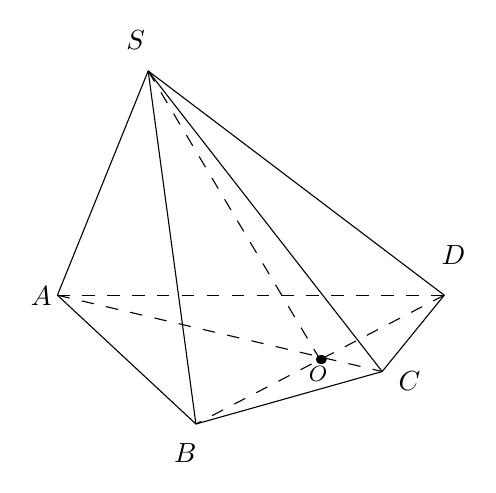
\begin{tikzpicture}[x=0.75pt,y=0.75pt,yscale=-1,xscale=1]
	%uncomment if require: \path (0,300); %set diagram left start at 0, and has height of 300
	
	%Straight Lines [id:da7583493554957284] 
	\draw  [dash pattern={on 4.5pt off 4.5pt}]  (242.11,141.19) -- (428.49,141.19) ;
	%Straight Lines [id:da459427114253375] 
	\draw    (242.11,141.19) -- (308.84,203.26) ;
	%Straight Lines [id:da38835471163621405] 
	\draw    (308.84,203.26) -- (398.58,177.97) ;
	%Straight Lines [id:da7752757632119569] 
	\draw    (428.49,141.19) -- (398.58,177.97) ;
	%Straight Lines [id:da34673079979599275] 
	\draw    (285.83,33.14) -- (242.11,141.19) ;
	%Straight Lines [id:da6105967556778404] 
	\draw    (285.83,33.14) -- (308.84,203.26) ;
	%Straight Lines [id:da3177261723711975] 
	\draw    (285.83,33.14) -- (398.58,177.97) ;
	%Straight Lines [id:da16389500438618199] 
	\draw    (285.83,33.14) -- (428.49,141.19) ;
	%Straight Lines [id:da5527613094130652] 
	\draw  [dash pattern={on 4.5pt off 4.5pt}]  (428.49,141.19) -- (308.84,203.26) ;
	%Straight Lines [id:da8942122896043776] 
	\draw  [dash pattern={on 4.5pt off 4.5pt}]  (242.11,141.19) -- (398.58,177.97) ;
	%Straight Lines [id:da12546053103631927] 
	\draw  [dash pattern={on 4.5pt off 4.5pt}]  (285.83,33.14) -- (368.67,172.23) ;
	%Shape: Free Drawing [id:dp6577929885295526] 
	\draw  [line width=3] [line join = round][line cap = round] (368.67,172.23) .. controls (369.05,172.23) and (369.43,172.23) .. (369.82,172.23) ;
	
	% Text Node
	\draw (274.08,12.57) node [anchor=north west][inner sep=0.75pt]   [align=left] {$S$};
	% Text Node
	\draw (228.05,135.56) node [anchor=north west][inner sep=0.75pt]   [align=left] {$A$};
	% Text Node
	\draw (297.09,211.43) node [anchor=north west][inner sep=0.75pt]   [align=left] {$B$};
	% Text Node
	\draw (405.24,176.95) node [anchor=north west][inner sep=0.75pt]   [align=left] {$C$};
	% Text Node
	\draw (425.95,116.02) node [anchor=north west][inner sep=0.75pt]   [align=left] {$D$};
	% Text Node
	\draw (362,174) node [anchor=north west][inner sep=0.75pt]  [font=\footnotesize] [align=left] {$O$};
	
	
\end{tikzpicture}
		\end{center}
	$\heva{&S\in (SAC) \\&S\in (SBD)}\Rightarrow S$ là điểm chung thứ nhất.\\
		$\heva{
			&O\in AC\subset\left(SAC\right)\\
			&O\in BD\subset\left(SBD\right)}$  $ \Rightarrow O$ là điểm chung thứ hai.\\
		Vậy $\left(SAC\right)\cap\left(SBD\right)=SO$.
}
\end{ex}

\begin{ex}%[1H4H1-3]Câu 3
	Cho hình chóp $ S.ABCD$ có đáy là hình thang $ ABCD\,(AB\parallel CD)$. Khẳng định nào sau đây {\bf sai}?
	\choice
	{Hình chóp $ S.ABCD$ có 4 mặt bên}
	{Giao tuyến của hai mặt phẳng $\left(SAC\right)$ và $\left(SBD\right)$ là $SO$ ($O$ là giao điểm của $AC$ và $BD$)}
	{Giao tuyến của hai mặt phẳng $\left(SAD\right)$ và $\left(SBC\right)$ là $SI$ ($I$ là giao điểm của $AD$ và $BC$)}
	{\True Giao tuyến của hai mặt phẳng $\left(SAB\right)$ và $\left(SAD\right)$ là đường trung bình của $ ABCD$}
	\loigiai{
	\begin{center}
		
		
		\tikzset{every picture/.style={line width=0.75pt}} %set default line width to 0.75pt        
		
		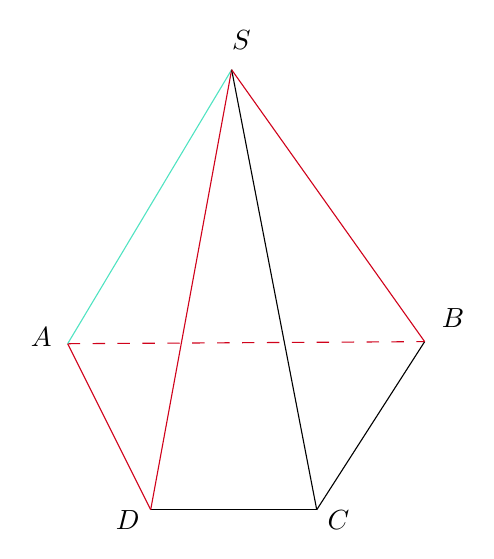
\begin{tikzpicture}[x=0.75pt,y=0.75pt,yscale=-1,xscale=1]
			%uncomment if require: \path (0,300); %set diagram left start at 0, and has height of 300
			
			%Straight Lines [id:da575608178282691] 
			\draw [color={rgb, 255:red, 208; green, 2; blue, 27 }  ,draw opacity=1 ] [dash pattern={on 4.5pt off 4.5pt}]  (152,176) -- (324,175) ;
			%Straight Lines [id:da4248466339274348] 
			\draw [color={rgb, 255:red, 208; green, 2; blue, 27 }  ,draw opacity=1 ]   (152,176) -- (192,256) ;
			%Straight Lines [id:da9556175916709888] 
			\draw    (324,175) -- (272,256) ;
			%Straight Lines [id:da45039350864708183] 
			\draw    (192,256) -- (272,256) ;
			%Straight Lines [id:da26541775038224347] 
			\draw [color={rgb, 255:red, 80; green, 227; blue, 194 }  ,draw opacity=1 ]   (231,44) -- (152,176) ;
			%Straight Lines [id:da10496555760002813] 
			\draw [color={rgb, 255:red, 208; green, 2; blue, 27 }  ,draw opacity=1 ]   (231,44) -- (192,256) ;
			%Straight Lines [id:da12955671213084963] 
			\draw    (231,44) -- (272,256) ;
			%Straight Lines [id:da28109086225514135] 
			\draw [color={rgb, 255:red, 208; green, 2; blue, 27 }  ,draw opacity=1 ]   (231,44) -- (324,175) ;
			
			% Text Node
			\draw (230,24) node [anchor=north west][inner sep=0.75pt]   [align=left] {$S$};
			% Text Node
			\draw (133,167) node [anchor=north west][inner sep=0.75pt]   [align=left] {$A$};
			% Text Node
			\draw (331,158) node [anchor=north west][inner sep=0.75pt]   [align=left] {$B$};
			% Text Node
			\draw (174,255) node [anchor=north west][inner sep=0.75pt]   [align=left] {$D$};
			% Text Node
			\draw (276,255) node [anchor=north west][inner sep=0.75pt]   [align=left] {$C$};
		\end{tikzpicture}
	\end{center}
	Ta có $\heva{&A\in (SAB)\\&A\in (SAD)}$ $\Rightarrow A$ là điểm chung thứ nhất.\\
	$\heva{&A\in (SAB)\\&A\in (SAD)}$ $\Rightarrow A$ là điểm chung thứ 2.\\
	Do đó $SA$ là giao tuyển của 2 mặt phẳng $\left(SAB\right)$ và $\left(SAD\right)$. }
\end{ex}
\begin{ex}%[1H4H1-3]Câu 4
	Cho hình chóp $ S.ABCD$, đáy $ ABCD$ là hình bình hành $ ABCD$ tâm $ O$. Giao tuyến của hai mặt phẳng $\left(SAC\right)$ và $\left(SAD\right)$ là
	\choice
	{$SO$}
	{$SD$}
	{\True $SA$}
	{$SB$}
	\loigiai{
			Ta có $\heva{&A\in (SAC)\\&A\in (SAD)}$ $\Rightarrow A$ là điểm chung thứ nhất.\\
		$\heva{&A\in (SAC)\\&A\in (SAD)}$ $\Rightarrow A$ là điểm chung thứ 2.\\
		Do đó $SA$ là giao tuyển của 2 mặt phẳng $\left(SAC\right)$ và $\left(SAD\right)$.
	}
\end{ex}

\begin{ex}%[1H4H1-3]Câu 5
	Cho tứ diện $ ABC{\rm{D}}$, $ G$ là trọng tâm tam giác $ BCD$. Giao tuyến của $\left(ACD\right)$ và $\left(GAB\right)$ là
	\choice
	{$ AM$ (với $ M$ là trung điểm $ AB$)}
	{\True $ AN$ (với $ N$ là trung điểm $ CD$)}
	{$ AK$ (với $ K$ là hình chiếu của $ C$ trên $ BD$)}
	{$ AH$ (với $ H$ là hình chiếu của $ B$ trên $CD$)}
	\loigiai{
		\begin{center}
			\tikzset{every picture/.style={line width=0.75pt}} %set default line width to 0.75pt        
			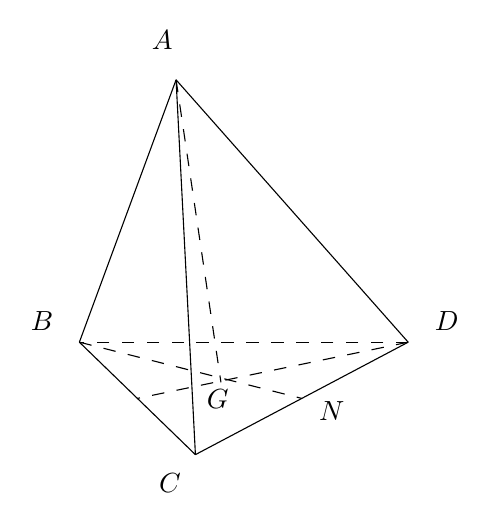
\begin{tikzpicture}[x=0.75pt,y=0.75pt,yscale=-1,xscale=1]
				%uncomment if require: \path (0,300); %set diagram left start at 0, and has height of 300
				
				%Straight Lines [id:da07685026365288206] 
				\draw  [dash pattern={on 4.5pt off 4.5pt}]  (378.21,169.61) -- (219.79,169.61) ;
				%Straight Lines [id:da9860254266492514] 
				\draw    (219.79,169.61) -- (275.7,223.79) ;
				%Straight Lines [id:da2894736661983659] 
				\draw    (266.38,43.21) -- (219.79,169.61) ;
				%Straight Lines [id:da3151259352492011] 
				\draw    (266.38,43.21) -- (275.7,223.79) ;
				%Straight Lines [id:da03911191486486554] 
				\draw    (266.38,43.21) -- (378.21,169.61) ;
				%Straight Lines [id:da545522614655316] 
				\draw  [dash pattern={on 4.5pt off 4.5pt}]  (219.79,169.61) -- (326.96,196.7) ;
				%Straight Lines [id:da03964216052894409] 
				\draw    (378.21,169.61) -- (275.7,223.79) ;
				%Straight Lines [id:da5856241460809652] 
				\draw  [dash pattern={on 4.5pt off 4.5pt}]  (378.21,169.61) -- (247.75,196.7) ;
				%Straight Lines [id:da21130713332169915] 
				\draw  [dash pattern={on 4.5pt off 4.5pt}]  (266.38,43.21) -- (288,189) ;
				
				% Text Node
				\draw (253.4,18.35) node [anchor=north west][inner sep=0.75pt]   [align=left] {$A$};
				% Text Node
				\draw (195.15,153.78) node [anchor=north west][inner sep=0.75pt]   [align=left] {$B$};
				% Text Node
				\draw (256.97,231.65) node [anchor=north west][inner sep=0.75pt]   [align=left] {$C$};
				% Text Node
				\draw (389.76,153.78) node [anchor=north west][inner sep=0.75pt]   [align=left] {$D$};
				% Text Node
				\draw (280,191) node [anchor=north west][inner sep=0.75pt]   [align=left] {$G$};
				% Text Node
				\draw (334,197) node [anchor=north west][inner sep=0.75pt]   [align=left] {$N$};				
			\end{tikzpicture}
		\end{center}
		Vì $G$ là trọng tâm tam giác $BCD$ nên gọi $N$ là trung điểm của $CD$.\\
		$\heva{&N\in BG, BG\subset (ABG)\Rightarrow N\in (ABG)\\&N \in CD \Rightarrow N\in (ACD)}\Rightarrow N$ là điểm chung thứ nhất.\\
		 $\heva{&A\in (ABG)\\&A\in (ACD)}$ $\Rightarrow A$ là điểm chung thứ hai\\.
		Ta thấy $\left(GAB\right)$ chính là mặt phẳng $\left(ANB\right)$. Suy ra giao tuyến của $\left(GAB\right)$ với $\left(AC{\rm{D}}\right)$ chính là $ AN$.}
\end{ex}

\begin{ex}%[1H4H2-4]Câu 6
	Cho hình chóp $ S.ABC$. Gọi $ M$ là trung điểm $ SA$; $N$ và $P$ lần lượt là điểm bất kì trên cạnh $ SB$, $ SC$ (không trùng với trung điểm và hai đầu mút). Giao điểm của $ MN$ với $\left(ABC\right)$ là
	\choice
	{giao điểm của $ MN$ với $ BC$}
	{giao điểm của $ MP$ với $ BC$}
	{\True giao điểm của $ MN$ với $ AB$}
	{giao điểm của $ MP$ với $ AC$}
	\loigiai{
	\begin{center}
		\tikzset{every picture/.style={line width=0.75pt}} %set default line width to 0.75pt        		
		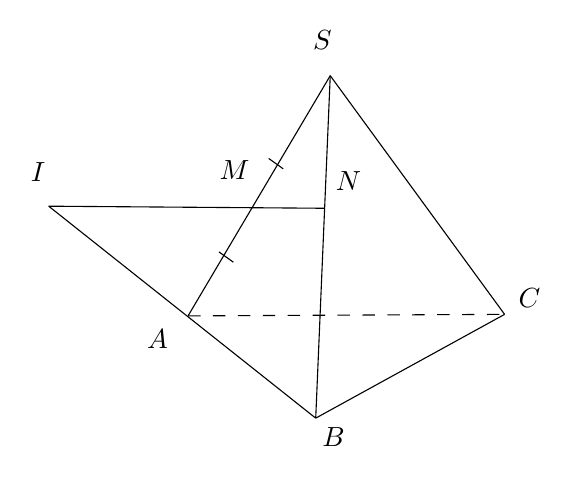
\begin{tikzpicture}[x=0.75pt,y=0.75pt,yscale=-1,xscale=1]
			%uncomment if require: \path (0,300); %set diagram left start at 0, and has height of 300
			
			%Straight Lines [id:da47172093832542683] 
			\draw  [dash pattern={on 4.5pt off 4.5pt}]  (224,161) -- (376.51,160.26) ;
			%Straight Lines [id:da26093450664971973] 
			\draw    (156.86,108.14) -- (285.51,210.26) ;
			%Straight Lines [id:da9080950852780671] 
			\draw    (376.51,160.26) -- (285.51,210.26) ;
			%Straight Lines [id:da508342626341979] 
			\draw    (292.51,45.26) -- (376.51,160.26) ;
			%Straight Lines [id:da5997859657126805] 
			\draw    (292.51,45.26) -- (285.51,210.26) ;
			%Straight Lines [id:da6156882522581331] 
			\draw    (292.51,45.26) -- (224,161) ;
			%Straight Lines [id:da21398720544529026] 
			\draw    (156.86,108.14) -- (289.86,109.14) ;
			%Straight Lines [id:da6515493276053881] 
			\draw    (262.86,85.14) -- (269.86,90.14) ;
			%Straight Lines [id:da28640410491758317] 
			\draw    (238.86,130.14) -- (245.86,135.14) ;
			
			% Text Node
			\draw (283,22.4) node [anchor=north west][inner sep=0.75pt]    {$S$};
			% Text Node
			\draw (287.51,213.66) node [anchor=north west][inner sep=0.75pt]    {$B$};
			% Text Node
			\draw (382,146.4) node [anchor=north west][inner sep=0.75pt]    {$C$};
			% Text Node
			\draw (203,166.4) node [anchor=north west][inner sep=0.75pt]    {$A$};
			% Text Node
			\draw (147,86) node [anchor=north west][inner sep=0.75pt]   [align=left] {$I$};
			% Text Node
			\draw (238,85) node [anchor=north west][inner sep=0.75pt]   [align=left] {$M$};
			% Text Node
			\draw (294,90) node [anchor=north west][inner sep=0.75pt]   [align=left] {$N$};
		\end{tikzpicture}
	\end{center}
		Trong $\left(SAB\right)$,$ MN\cap AB=\left\{ I\right\}\Rightarrow
		\heva{&I\in MN\\&
			I\in AB\Rightarrow I\in\left(ABC\right)}$
		 $\Rightarrow MN\cap\left(ABC\right)=\left\{ I\right\}$.\\
		Vậy giao điểm của $ MN$ với $\left(ABC\right)$ là giao điểm của $ MN$ với $ AB$.}
\end{ex}

\begin{ex}%[1H4H2-4]Câu 7
	Cho tứ diện $ ABCD$. Lấy điểm $ M$ sao cho $ AM=2CM$ và $ N$ là trung điểm $ AD$. Gọi $ O$ là một điểm thuộc miền trong của $\triangle BCD$. Giao điểm của $ BC$ với $\left(OMN\right)$ là giao điểm của $ BC$ với
	\choice
	{$OM$}
	{$MN$}
	{$OM,MN$ đều đúng}
	{\True $OM,MN$ đều sai}
	\loigiai{
\begin{center}
	
	
	\tikzset{every picture/.style={line width=0.75pt}} %set default line width to 0.75pt        
	
	\begin{tikzpicture}[x=0.75pt,y=0.75pt,yscale=-1,xscale=1]
		%uncomment if require: \path (0,300); %set diagram left start at 0, and has height of 300
		
		%Straight Lines [id:da47172093832542683] 
		\draw  [dash pattern={on 4.5pt off 4.5pt}]  (231.51,183.01) -- (435.21,182.15) ;
		%Straight Lines [id:da26093450664971973] 
		\draw    (231.51,183.01) -- (313.67,239.88) ;
		%Straight Lines [id:da9080950852780671] 
		\draw    (435.21,182.15) -- (313.67,239.88) ;
		%Straight Lines [id:da508342626341979] 
		\draw    (323.02,49.37) -- (435.21,182.15) ;
		%Straight Lines [id:da5997859657126805] 
		\draw    (323.02,49.37) -- (313.67,239.88) ;
		%Straight Lines [id:da6156882522581331] 
		\draw    (323.02,49.37) -- (231.51,183.01) ;
		%Straight Lines [id:da2900084067950517] 
		\draw    (273.31,121.16) -- (317.92,169.97) ;
		%Straight Lines [id:da02934092155698731] 
		\draw  [dash pattern={on 4.5pt off 4.5pt}]  (273.31,121.16) -- (285.77,201.03) ;
		%Straight Lines [id:da9829417668842391] 
		\draw  [dash pattern={on 4.5pt off 4.5pt}]  (317.92,169.97) -- (285.77,201.03) ;
		
		% Text Node
		\draw (203.49,174.61) node [anchor=north west][inner sep=0.75pt]    {$D$};
		% Text Node
		\draw (446.93,165.39) node [anchor=north west][inner sep=0.75pt]    {$B$};
		% Text Node
		\draw (309.42,244.98) node [anchor=north west][inner sep=0.75pt]    {$C$};
		% Text Node
		\draw (317.34,29.29) node [anchor=north west][inner sep=0.75pt]    {$A$};
		% Text Node
		\draw (257.5,105.82) node [anchor=north west][inner sep=0.75pt]   [align=left] {N};
		% Text Node
		\draw (282.22,199.81) node [anchor=north west][inner sep=0.75pt]   [align=left] {O};
		% Text Node
		\draw (323.31,153.16) node [anchor=north west][inner sep=0.75pt]   [align=left] {M};
	\end{tikzpicture}
\end{center}
		Dễ thấy $ OM$ không đồng phẳng với $ BC$ và $ MN$ cũng không đồng phẳng với $ BC$. Vậy cả $OM$ và $MN$ đều sai.}
\end{ex}

\begin{ex}%[1H4H2-4]Câu 8
	Cho tứ diện $ ABCD$. Gọi $ M$ và $ N$ lần lượt là trung điểm của $ BC$ và $ AD$; $ G$ là trung điểm của $ MN$. Trong các khẳng định sau, khẳng định nào {\bf sai}?
	\choice
	{$ BG\cap\left(ACD\right)=B'\,\,;\,\,B'$ là trọng tâm tam giác $ ACD$}
	{$ G$ là trọng tâm tứ diện $ ABCD$}
	{$ AG\cap\left(BCD\right)=A'\,\,;\,\,A'$ là trọng tâm tam giác $ BCD$}
	{\True $ G$ là trọng tâm tam giác $ ADM$}
	\loigiai{
		\begin{center}	
	\tikzset{every picture/.style={line width=0.75pt}} %set default line width to 0.75pt        
	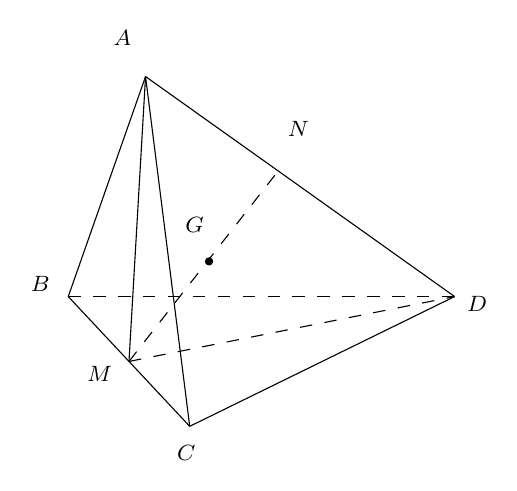
\begin{tikzpicture}[x=0.75pt,y=0.75pt,yscale=-1,xscale=1]
		%uncomment if require: \path (0,300); %set diagram left start at 0, and has height of 300
		
		%Straight Lines [id:da48129746659918693] 
		\draw  [dash pattern={on 4.5pt off 4.5pt}]  (231.6,157.55) -- (417.75,157.55) ;
		%Straight Lines [id:da8422554368974069] 
		\draw    (231.6,157.55) -- (290.11,220.07) ;
		%Straight Lines [id:da437222355451675] 
		\draw    (417.75,157.55) -- (290.11,220.07) ;
		%Straight Lines [id:da6503059809783438] 
		\draw    (231.6,157.55) -- (268.83,51.54) ;
		%Straight Lines [id:da1487688114216692] 
		\draw    (268.83,51.54) -- (290.11,220.07) ;
		%Straight Lines [id:da9186344685038683] 
		\draw    (268.83,51.54) -- (417.75,157.55) ;
		%Straight Lines [id:da8575371812933177] 
		\draw    (268.83,51.54) -- (260.85,188.81) ;
		%Straight Lines [id:da2759693358784179] 
		\draw  [dash pattern={on 4.5pt off 4.5pt}]  (260.85,188.81) -- (326.76,175.68) -- (417.75,157.55) ;
		%Straight Lines [id:da6729739085721969] 
		\draw  [dash pattern={on 4.5pt off 4.5pt}]  (260.85,188.81) -- (332.68,97.11) ;
		%Shape: Free Drawing [id:dp8048355646753238] 
		\draw  [line width=3] [line join = round][line cap = round] (299.44,140.6) .. controls (299.44,140.6) and (299.44,140.6) .. (299.44,140.6) ;
		
		% Text Node
		\draw (252.2,28.27) node [anchor=north west][inner sep=0.75pt]  [font=\footnotesize]  {$A$};
		% Text Node
		\draw (212.31,146.51) node [anchor=north west][inner sep=0.75pt]  [font=\footnotesize]  {$B$};
		% Text Node
		\draw (336.12,71.76) node [anchor=north west][inner sep=0.75pt]  [font=\footnotesize]  {$N$};
		% Text Node
		\draw (282.78,228.06) node [anchor=north west][inner sep=0.75pt]  [font=\footnotesize]  {$C$};
		% Text Node
		\draw (239.39,190) node [anchor=north west][inner sep=0.75pt]  [font=\footnotesize]  {$M$};
		% Text Node
		\draw (422.55,156.03) node [anchor=north west][inner sep=0.75pt]  [font=\footnotesize]  {$D$};
		% Text Node
		\draw (286.76,117.97) node [anchor=north west][inner sep=0.75pt]  [font=\footnotesize]  {$G$};		
	\end{tikzpicture}
		\end{center}
		Xét tam giác $ ADM$ có $ MN$ là đường trung tuyến.\\
		Do $ G$ là trung điểm của $ MN$ $\Rightarrow G$ không là trọng tâm của tam giác $ ADM$.}
\end{ex}

\begin{ex}%[1H4V2-5]Câu 9
	Cho hình chóp $S.ABCD$ có đáy $ABCD$ là hình bình hành. Gọi $M$, $N$, $P$ lần lượt là trung điểm của $SA$, $SB$, $SC$. Thiết diện của hình chóp $S.ABCD$ cắt bởi mặt phẳng $(MNP)$ là
	\choice
	{\True Tứ giác}
	{Tam giác}
	{Ngũ giác}
	{Lục giác}
	\loigiai{
	\begin{center}
		
		
		\tikzset{every picture/.style={line width=0.75pt}} %set default line width to 0.75pt        
		
		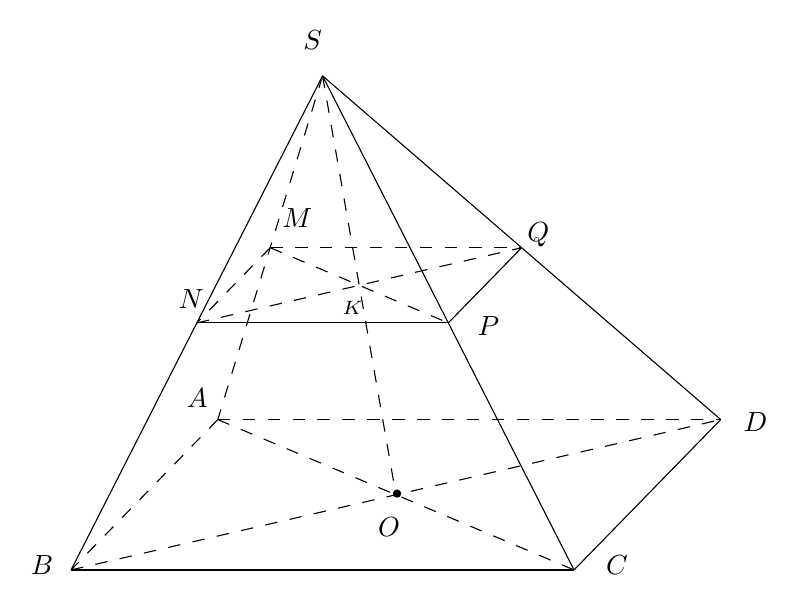
\begin{tikzpicture}[x=0.75pt,y=0.75pt,yscale=-1,xscale=1]
			%uncomment if require: \path (0,300); %set diagram left start at 0, and has height of 300
			
			%Straight Lines [id:da4881092025141185] 
			\draw  [dash pattern={on 4.5pt off 4.5pt}]  (163.12,202.05) -- (405.44,202.05) ;
			%Straight Lines [id:da9335098600184679] 
			\draw    (92.44,274.5) -- (334.76,274.5) ;
			%Straight Lines [id:da3070296527576508] 
			\draw  [dash pattern={on 4.5pt off 4.5pt}]  (163.12,202.05) -- (92.44,274.5) ;
			%Straight Lines [id:da7402066895693273] 
			\draw    (405.44,202.05) -- (334.76,274.5) ;
			%Straight Lines [id:da06492206227408404] 
			\draw  [dash pattern={on 4.5pt off 4.5pt}]  (213.6,36.45) -- (163.12,202.05) ;
			%Straight Lines [id:da9059384928905383] 
			\draw    (213.6,36.45) -- (92.44,274.5) ;
			%Straight Lines [id:da4785448923512914] 
			\draw    (213.6,36.45) -- (405.44,202.05) ;
			%Straight Lines [id:da8155686646377747] 
			\draw    (213.6,36.45) -- (334.76,274.5) ;
			%Straight Lines [id:da4257751792768276] 
			\draw  [dash pattern={on 4.5pt off 4.5pt}]  (163.12,202.05) -- (334.76,274.5) ;
			%Straight Lines [id:da743137678151826] 
			\draw  [dash pattern={on 4.5pt off 4.5pt}]  (92.44,274.5) -- (405.44,202.05) ;
			%Straight Lines [id:da18748296686017096] 
			\draw  [dash pattern={on 4.5pt off 4.5pt}]  (213.6,36.45) -- (248.94,238.27) ;
			%Shape: Free Drawing [id:dp2686464034677083] 
			\draw  [line width=3] [line join = round][line cap = round] (249.5,237.7) .. controls (249.5,237.7) and (249.5,237.7) .. (249.5,237.7) ;
			%Straight Lines [id:da4816981926432744] 
			\draw  [dash pattern={on 4.5pt off 4.5pt}]  (188.36,119.25) -- (309.52,119.25) ;
			%Straight Lines [id:da038122418353590426] 
			\draw    (153.02,155.48) -- (274.18,155.48) ;
			%Straight Lines [id:da6691879829704848] 
			\draw  [dash pattern={on 4.5pt off 4.5pt}]  (188.36,119.25) -- (153.02,155.48) ;
			%Straight Lines [id:da3131283071033737] 
			\draw    (309.52,119.25) -- (274.18,155.48) ;
			%Straight Lines [id:da6510790651179053] 
			\draw  [dash pattern={on 4.5pt off 4.5pt}]  (188.36,119.25) -- (274.18,155.48) ;
			%Straight Lines [id:da18303018708548824] 
			\draw  [dash pattern={on 4.5pt off 4.5pt}]  (153.02,155.48) -- (309.52,119.25) ;
			
			% Text Node
			\draw (203.05,13.5) node [anchor=north west][inner sep=0.75pt]   [align=left] {$S$};
			% Text Node
			\draw (146.96,186) node [anchor=north west][inner sep=0.75pt]   [align=left] {$A$};
			% Text Node
			\draw (71.79,266.5) node [anchor=north west][inner sep=0.75pt]   [align=left] {$B$};
			% Text Node
			\draw (348.96,266.5) node [anchor=north west][inner sep=0.75pt]   [align=left] {$C$};
			% Text Node
			\draw (415.15,197.5) node [anchor=north west][inner sep=0.75pt]   [align=left] {$D$};
			% Text Node
			\draw (239.07,248.1) node [anchor=north west][inner sep=0.75pt]   [align=left] {$O$};
			% Text Node
			\draw (222,144) node [anchor=north west][inner sep=0.75pt]  [font=\scriptsize] [align=left] {\textbf{$K$}};
			% Text Node
			\draw (193,99) node [anchor=north west][inner sep=0.75pt]   [align=left] {$M$};
			% Text Node
			\draw (143,138) node [anchor=north west][inner sep=0.75pt]   [align=left] {$N$};
			% Text Node
			\draw (311,106) node [anchor=north west][inner sep=0.75pt]   [align=left] {$Q$};
			% Text Node
			\draw (287,151) node [anchor=north west][inner sep=0.75pt]   [align=left] {$P$};
		\end{tikzpicture}
	\end{center}
		Gọi $ O=AC\cap BD$ và $ K=SO\cap MP$. Khi đó $NK$ cắt $SD$. Gọi $ Q=NK\cap SD$.\\
		Ta có $ (MNPQ)\equiv (MNP)\Rightarrow $ Thiết diện của hình chóp $S.ABCD$ cắt bởi mặt phẳng $(MNP)$ là tứ giác $MNPQ$.}
\end{ex}

\begin{ex}%[1H4H2-5]Câu 10
	Cho hình chóp $ S.ABCD$ có đáy $ ABCD$ là hình bình hành. Gọi $ I$, $ J$, $ K$ lần lượt là trung điểm các cạnh $ SA$, $ BC$, $ CD$. Thiết diện của $ S.ABCD$ cắt bởi mặt phẳng $\left(IJK\right)$ là
	\choice
	{Hình tam giác}
	{\True Hình ngũ giác}
	{Hình lục giác}
	{Hình tứ giác}
	\loigiai{
		\begin{center}
			
			
			\tikzset{every picture/.style={line width=0.75pt}} %set default line width to 0.75pt        
			
			\begin{tikzpicture}[x=0.75pt,y=0.75pt,yscale=-1,xscale=1]
				%uncomment if require: \path (0,300); %set diagram left start at 0, and has height of 300
				
				%Straight Lines [id:da2694434756888451] 
				\draw    (256,208) -- (360,208) ;
				%Straight Lines [id:da4139158770830369] 
				\draw  [dash pattern={on 4.5pt off 4.5pt}]  (191,159) -- (95,245) ;
				%Straight Lines [id:da9709608084514567] 
				\draw  [dash pattern={on 4.5pt off 4.5pt}]  (191,157) -- (416,160) ;
				%Straight Lines [id:da7858139098697641] 
				\draw    (388,184) -- (360,208) ;
				%Straight Lines [id:da3544794441636292] 
				\draw  [dash pattern={on 4.5pt off 4.5pt}]  (223,47) -- (191,159) ;
				%Straight Lines [id:da3963022482699823] 
				\draw  [dash pattern={on 4.5pt off 4.5pt}]  (165,155) -- (136,208) ;
				%Straight Lines [id:da6100422581341887] 
				\draw    (224,48) -- (360,208) ;
				%Straight Lines [id:da07672146619763587] 
				\draw    (224,48) -- (360,128) ;
				%Straight Lines [id:da8362640849835135] 
				\draw  [dash pattern={on 4.5pt off 4.5pt}]  (208,104) -- (388,184) ;
				%Straight Lines [id:da9061732422205897] 
				\draw  [dash pattern={on 4.5pt off 4.5pt}]  (207,101) -- (255,205) ;
				%Straight Lines [id:da200996237593148] 
				\draw [color={rgb, 255:red, 208; green, 2; blue, 27 }  ,draw opacity=1 ]   (388,184) -- (256,208) ;
				%Straight Lines [id:da8673730868303331] 
				\draw    (256,208) -- (24,256) ;
				%Straight Lines [id:da47629695761441937] 
				\draw    (616,136) -- (384,184) ;
				%Straight Lines [id:da011767740496870127] 
				\draw [color={rgb, 255:red, 208; green, 2; blue, 27 }  ,draw opacity=1 ] [dash pattern={on 4.5pt off 4.5pt}]  (207,103) -- (359,127) ;
				%Straight Lines [id:da3147473883726344] 
				\draw [color={rgb, 255:red, 208; green, 2; blue, 27 }  ,draw opacity=1 ] [dash pattern={on 4.5pt off 4.5pt}]  (165,155) -- (207,103) ;
				%Straight Lines [id:da09185657215699194] 
				\draw    (100,240) -- (165,155) ;
				%Straight Lines [id:da08891440246072246] 
				\draw    (360,128) -- (495,160) ;
				%Straight Lines [id:da9748156246999811] 
				\draw [color={rgb, 255:red, 208; green, 2; blue, 27 }  ,draw opacity=1 ]   (165,155) -- (256,208) ;
				%Straight Lines [id:da10451458247112022] 
				\draw [color={rgb, 255:red, 208; green, 2; blue, 27 }  ,draw opacity=1 ]   (360,128) -- (388,184) ;
				%Straight Lines [id:da062279200426914594] 
				\draw  [dash pattern={on 4.5pt off 4.5pt}]  (416,160) -- (495,160) ;
				%Straight Lines [id:da14630119480240777] 
				\draw    (223,47) -- (165,155) ;
				%Straight Lines [id:da026754655289340068] 
				\draw  [dash pattern={on 4.5pt off 4.5pt}]  (136,208) -- (256,208) ;
				%Straight Lines [id:da1872974965918568] 
				\draw  [dash pattern={on 4.5pt off 4.5pt}]  (416,160) -- (388,184) ;
				%Straight Lines [id:da8971324037253503] 
				\draw  [dash pattern={on 4.5pt off 4.5pt}]  (359,127) -- (416,160) ;
				
				% Text Node
				\draw (216,22) node [anchor=north west][inner sep=0.75pt]   [align=left] {$S$};
				% Text Node
				\draw (219,82) node [anchor=north west][inner sep=0.75pt]   [align=left] {$I$};
				% Text Node
				\draw (201,137) node [anchor=north west][inner sep=0.75pt]   [align=left] {$A$};
				% Text Node
				\draw (138,211) node [anchor=north west][inner sep=0.75pt]   [align=left] {$B$};
				% Text Node
				\draw (346,212) node [anchor=north west][inner sep=0.75pt]   [align=left] {$C$};
				% Text Node
				\draw (416,142) node [anchor=north west][inner sep=0.75pt]   [align=left] {$D$};
				% Text Node
				\draw (91,221) node [anchor=north west][inner sep=0.75pt]   [align=left] {$N$};
				% Text Node
				\draw (495,141) node [anchor=north west][inner sep=0.75pt]   [align=left] {$M$};
				% Text Node
				\draw (148,142) node [anchor=north west][inner sep=0.75pt]   [align=left] {$F$};
				% Text Node
				\draw (358,107) node [anchor=north west][inner sep=0.75pt]   [align=left] {$E$};
				% Text Node
				\draw (258,211) node [anchor=north west][inner sep=0.75pt]   [align=left] {$J$};
				% Text Node
				\draw (390,187) node [anchor=north west][inner sep=0.75pt]   [align=left] {$K$};
				
				
			\end{tikzpicture}
		\end{center}
		Gọi $ M=JK\cap AD$, $ N=JK\cap AB$, $ F=IN\cap SB$ và $ E=IM\cap SD$.\\
		Khi đó, mặt phẳng $\left(IJK\right)$ cắt hình chóp $ S.ABCD$ theo thiết diện là ngũ giác $ IFJKE$.}
\end{ex}

\begin{ex}%[1H4H2-5]Câu 11
	Cho tứ diện $ ABCD$. Gọi $ H,K$ lần lượt là trung điểm các cạnh $AB,AC$. Trên đường thẳng $ CD$ lấy điểm $ M$ nằm ngoài đoạn $ CD$. Thiết diện của tứ diện với mặt phẳng $ (HKM)$ là
	\choice
	{Tứ giác $ HKMN$ với $ N\in AD$}
	{Hình thang $ HKMN$ với $ N\in AD$ và $ HK//MN$}
	{\True Tam giác $ HKL$ với $ L=KM\cap AD$}
	{Tam giác $ HKL$ với $ L=HM\cap AD$}
	\loigiai{
		\begin{center}
	\tikzset{every picture/.style={line width=0.75pt}} %set default line width to 0.75pt        
	
	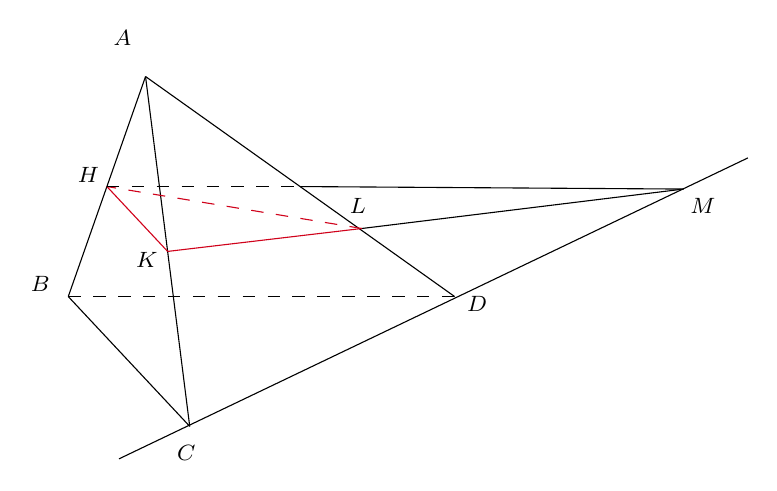
\begin{tikzpicture}[x=0.75pt,y=0.75pt,yscale=-1,xscale=1]
		%uncomment if require: \path (0,300); %set diagram left start at 0, and has height of 300
		
		%Straight Lines [id:da41557366413922026] 
		\draw  [dash pattern={on 4.5pt off 4.5pt}]  (231.6,157.55) -- (417.75,157.55) ;
		%Straight Lines [id:da9801382567934529] 
		\draw    (231.6,157.55) -- (290.11,220.07) ;
		%Straight Lines [id:da013183781835474306] 
		\draw    (559.02,90.76) -- (256.02,235.76) ;
		%Straight Lines [id:da5045134391073287] 
		\draw    (231.6,157.55) -- (268.83,51.54) ;
		%Straight Lines [id:da31363985783033455] 
		\draw    (268.83,51.54) -- (290.11,220.07) ;
		%Straight Lines [id:da27219218982545246] 
		\draw    (268.83,51.54) -- (417.75,157.55) ;
		%Straight Lines [id:da8043644679649002] 
		\draw [color={rgb, 255:red, 208; green, 2; blue, 27 }  ,draw opacity=1 ]   (250.22,104.55) -- (279.47,135.8) ;
		%Straight Lines [id:da945942871551033] 
		\draw    (373.02,124.76) -- (528.02,105.76) ;
		%Straight Lines [id:da26373425513408155] 
		\draw    (343.29,104.55) -- (528.02,105.76) ;
		%Straight Lines [id:da37850073453471733] 
		\draw [color={rgb, 255:red, 208; green, 2; blue, 27 }  ,draw opacity=1 ] [dash pattern={on 4.5pt off 4.5pt}]  (373.02,124.76) -- (250.22,104.55) ;
		%Straight Lines [id:da44154183798251334] 
		\draw  [dash pattern={on 4.5pt off 4.5pt}]  (250.22,104.55) -- (343.29,104.55) ;
		%Straight Lines [id:da0184408732547372] 
		\draw [color={rgb, 255:red, 208; green, 2; blue, 27 }  ,draw opacity=1 ]   (373.02,124.76) -- (279.47,135.8) ;
		
		% Text Node
		\draw (252.2,28.27) node [anchor=north west][inner sep=0.75pt]  [font=\footnotesize]  {$A$};
		% Text Node
		\draw (212.31,146.51) node [anchor=north west][inner sep=0.75pt]  [font=\footnotesize]  {$B$};
		% Text Node
		\draw (282.78,228.06) node [anchor=north west][inner sep=0.75pt]  [font=\footnotesize]  {$C$};
		% Text Node
		\draw (530.02,109.16) node [anchor=north west][inner sep=0.75pt]  [font=\footnotesize]  {$M$};
		% Text Node
		\draw (422.55,156.03) node [anchor=north west][inner sep=0.75pt]  [font=\footnotesize]  {$D$};
		% Text Node
		\draw (235,94.09) node [anchor=north west][inner sep=0.75pt]  [font=\footnotesize]  {$H$};
		% Text Node
		\draw (263,135.09) node [anchor=north west][inner sep=0.75pt]  [font=\footnotesize]  {$K$};
		% Text Node
		\draw (366,109.09) node [anchor=north west][inner sep=0.75pt]  [font=\footnotesize]  {$L$};		
	\end{tikzpicture}
		\end{center}
		Có $KM$ và $AD$ đồng phẳng trong mp$(ACD)$ và $KM$ cắt $AD$. Tức là\\
		$ (HKM)$ cắt $(ACD)$ theo đoạn giao tuyến $KL$.\\
		$ (HKM)$ cắt $(ABD)$ theo đoạn giao tuyến $HL$.\\
		Vậy thiết diện là tam giác $HKL$.}
\end{ex}

\begin{ex}%[1H4V2-6]Câu 12
	Cho hình tứ diện $ ABCD$ có $M$ , $N$ lần lượt là trung điểm của $AB$ , $BD$ . Các điểm $G$ , $H$ lần lượt trên cạnh $AC$ , $CD$ sao cho $NH$ cắt $MG$ tại $I$ . Khẳng định nào sau đây là khẳng định đúng?
	\choice
	{$ A$, $C$ , $I$ thẳng hàng}
	{\True $B$ , $ C$, $I$ thẳng hàng}
	{$ N$, $ G$, $H$ thẳng hàng}
	{$ B$, $G$ , $H$ thẳng hàng}
	\loigiai{
	\begin{center}
	
	
	\tikzset{every picture/.style={line width=0.75pt}} %set default line width to 0.75pt        
	
	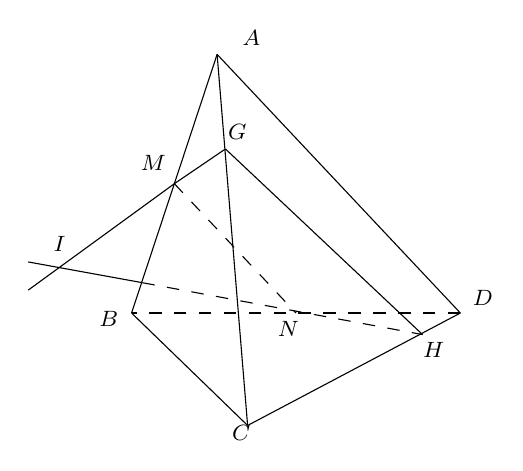
\begin{tikzpicture}[x=0.75pt,y=0.75pt,yscale=-1,xscale=1]
		%uncomment if require: \path (0,300); %set diagram left start at 0, and has height of 300
		
		%Straight Lines [id:da07685026365288206] 
		\draw  [dash pattern={on 4.5pt off 4.5pt}]  (378.21,169.61) -- (219.79,169.61) ;
		%Straight Lines [id:da9860254266492514] 
		\draw    (219.79,169.61) -- (275.7,223.79) ;
		%Straight Lines [id:da2894736661983659] 
		\draw    (261,45) -- (219.79,169.61) ;
		%Straight Lines [id:da3151259352492011] 
		\draw    (261,45) -- (275.7,223.79) ;
		%Straight Lines [id:da03911191486486554] 
		\draw    (261,45) -- (378.21,169.61) ;
		%Straight Lines [id:da03964216052894409] 
		\draw    (378.21,169.61) -- (275.7,223.79) ;
		%Straight Lines [id:da7695523174190944] 
		\draw  [dash pattern={on 4.5pt off 4.5pt}]  (240.4,107.31) -- (299,169.61) ;
		%Straight Lines [id:da5824753432796959] 
		\draw    (170.02,158.56) -- (240.4,107.31) -- (265.02,90.56) ;
		%Straight Lines [id:da26839968552406934] 
		\draw    (265.02,90.56) -- (360,180) ;
		%Straight Lines [id:da2576785961066459] 
		\draw  [dash pattern={on 4.5pt off 4.5pt}]  (225,155) -- (360,180) ;
		%Straight Lines [id:da14810069434258333] 
		\draw    (170,145) -- (225,155) ;
		
		% Text Node
		\draw (272,32.4) node [anchor=north west][inner sep=0.75pt]  [font=\footnotesize]  {$A$};
		% Text Node
		\draw (223,92.4) node [anchor=north west][inner sep=0.75pt]  [font=\footnotesize]  {$M$};
		% Text Node
		\draw (383,157.4) node [anchor=north west][inner sep=0.75pt]  [font=\footnotesize]  {$D$};
		% Text Node
		\draw (359,182.4) node [anchor=north west][inner sep=0.75pt]  [font=\footnotesize]  {$H$};
		% Text Node
		\draw (267,222.4) node [anchor=north west][inner sep=0.75pt]  [font=\footnotesize]  {$C$};
		% Text Node
		\draw (289,172.4) node [anchor=north west][inner sep=0.75pt]  [font=\footnotesize]  {$N$};
		% Text Node
		\draw (203,167.4) node [anchor=north west][inner sep=0.75pt]  [font=\footnotesize]  {$B$};
		% Text Node
		\draw (181,131.4) node [anchor=north west][inner sep=0.75pt]  [font=\footnotesize]  {$I$};
		% Text Node
		\draw (265,77.4) node [anchor=north west][inner sep=0.75pt]  [font=\footnotesize]  {$G$};
		
		
	\end{tikzpicture}
	\end{center}
		Do $ NH$ cắt $ MG$ tại $ I$ nên bốn điểm $ M,N,H,G$ cùng thuộc mặt phẳng $\left(\alpha\right)$. Xét ba mặt phẳng $\left(ABC\right)$, $\left(BCD\right)$, $\left(\alpha\right)$ phân biệt, đồng thời $\heva{
			&\left(\alpha\right)\cap\left(ABC\right)=MG\\
			&\left(\alpha\right)\cap\left(BCD\right)=NH\\
			&\left(ABC\right)\cap\left(BCD\right)=BC.}$\\
			Suy ra $ MG$, $ NH$, $\,BC$ đồng quy tại $ I$ nên $ B$, $ C$, $ I$ thẳng hàng.
}
	\end{ex}
\Closesolutionfile{ans}
\indapan{6}{ans/ans-0-B1}
\cauds
\Opensolutionfile{ans}[ans/ans-0-B1-DS]
\begin{ex}%[1H4H1-3]
Cho hình chóp $ S.ABCD$, biết $ AB$ cắt $ CD$ tại $ E,AC$ cắt $ BD$ tại $ F$ trong mặt phẳng đáy. Khi đó:
	\choiceTF
	{\True Đường thẳng $ EF$ nằm trong mặt phẳng $ (ABCD)$}
	{\True $ AB$ là giao tuyến của hai mặt phẳng $ (SAB)$ và $ (ABCD)$}
	{ $ SF$ là giao tuyến của hai mặt phẳng $ (SAB)$ và $ (SCD),$ $ SE$ là giao tuyến của hai mặt phẳng $ (SAC)$ và $ (SBD)$}
	{ Gọi $ G=EF\cap AD$ khi đó, $ SG$ giao tuyến của mặt phẳng $ (SEF)$ và mặt phẳng $ (SAD)$}
	\loigiai{
		\begin{itemchoice}
			\itemch Đúng. Ta có $ E=AB\cap CD\Rightarrow E\in AB,AB\subset (ABCD)\Rightarrow E\in (ABCD)$.\\
			Tương tự: $ F=AC\cap BD\Rightarrow F\in AC,AC\subset (ABCD)\Rightarrow F\in (ABCD)$. \\Vậy $ EF\subset (ABCD)$.
			\itemch  Sai. Dễ thấy $ A$ là điểm chung của hai mặt phẳng $ (SAB)$ và $ (ABCD),B$ cũng là điểm chung của hai mặt phẳng $ (SAB)$ và $ (ABCD)$.\\
			Suy ra $ AB=(SAB)\cap (ABCD)$.
			\begin{center}
				
				
				\tikzset{every picture/.style={line width=0.75pt}} %set default line width to 0.75pt        
				
				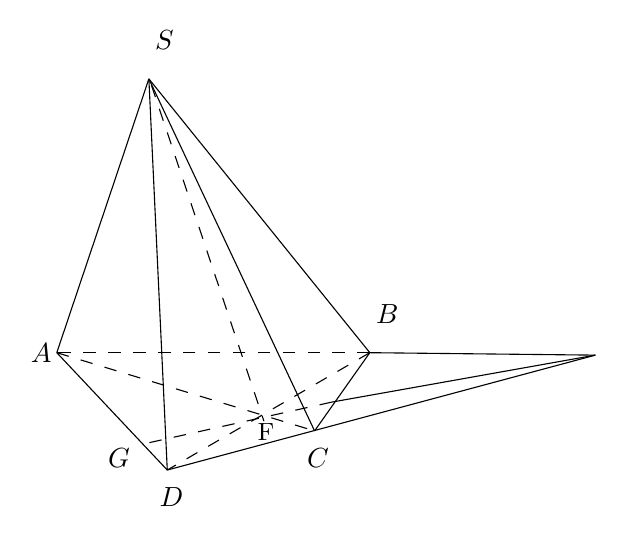
\begin{tikzpicture}[x=0.75pt,y=0.75pt,yscale=-1,xscale=1]
					%uncomment if require: \path (0,300); %set diagram left start at 0, and has height of 300
					
					%Straight Lines [id:da06829326789304124] 
					\draw  [dash pattern={on 4.5pt off 4.5pt}]  (368.33,176.19) -- (217.52,176.19) ;
					%Straight Lines [id:da4879034433791012] 
					\draw    (217.52,176.19) -- (270.75,232.73) ;
					%Straight Lines [id:da9140078445794462] 
					\draw    (477,177.37) -- (270.75,232.73) ;
					%Straight Lines [id:da2628600403292536] 
					\draw    (368.33,176.19) -- (341.72,213.88) ;
					%Straight Lines [id:da2812372111415704] 
					\draw    (261.88,44.27) -- (217.52,176.19) ;
					%Straight Lines [id:da4208975267964046] 
					\draw    (261.88,44.27) -- (270.75,232.73) ;
					%Straight Lines [id:da875180458786619] 
					\draw    (261.88,44.27) -- (341.72,213.88) ;
					%Straight Lines [id:da05187362756249869] 
					\draw    (261.88,44.27) -- (368.33,176.19) ;
					%Straight Lines [id:da3650664938160457] 
					\draw  [dash pattern={on 4.5pt off 4.5pt}]  (217.52,176.19) -- (299.85,201.18) -- (341.72,213.88) ;
					%Straight Lines [id:da14029076962674147] 
					\draw  [dash pattern={on 4.5pt off 4.5pt}]  (368.33,176.19) -- (270.75,232.73) ;
					%Straight Lines [id:da18406651080792513] 
					\draw  [dash pattern={on 4.5pt off 4.5pt}]  (263.12,47.34) -- (317.32,209.17) ;
					%Straight Lines [id:da94172605545418] 
					\draw    (368.33,176.19) -- (477,177.37) ;
					%Straight Lines [id:da84202281209602] 
					\draw    (477,177.37) -- (350,200) ;
					%Straight Lines [id:da9750296089145654] 
					\draw  [dash pattern={on 4.5pt off 4.5pt}]  (350,200) -- (260,220) ;
					
					% Text Node
					\draw (263.64,19.87) node [anchor=north west][inner sep=0.75pt]   [align=left] {$S$};
					% Text Node
					\draw (203.76,170.64) node [anchor=north west][inner sep=0.75pt]   [align=left] {$A$};
					% Text Node
					\draw (370.09,151.79) node [anchor=north west][inner sep=0.75pt]   [align=left] {$B$};
					% Text Node
					\draw (336.83,221.29) node [anchor=north west][inner sep=0.75pt]   [align=left] {$C$};
					% Text Node
					\draw (265.86,240.13) node [anchor=north west][inner sep=0.75pt]   [align=left] {$D$};
					% Text Node
					\draw (313,209) node [anchor=north west][inner sep=0.75pt]  [font=\small] [align=left] {F};
					% Text Node
					\draw (241,221) node [anchor=north west][inner sep=0.75pt]   [align=left] {$G$};
				\end{tikzpicture}
			\end{center}
			\itemch Đúng. Tìm giao tuyến của $ (SAB)$ và $ SCD)$ :\\
			Dễ thấy $ S$ là điểm chung của hai mặt phẳng $ (SAB)$ và $ (SCD)$.\\
			Ta có $\heva{
					&{E\in AB,AB\subset (SAB)}\\
					&{E\in CD,CD\subset (SCD)}
				.}$\\
			Vậy $ SE=(SAB)\cap (SCD)$.\\
			Tìm giao tuyến của $ (SAC)$ và $ (SBD)$ :\\
			Dễ thấy $ S$ là điểm chung của hai mặt phẳng $ (SAC)$ và $ (SBD)$.\\
			Ta có $\heva{
					&{F\in AC,AC\subset (SAC)}\\
				    &{F\in BD,BD\subset (SBD).}
				}$\\
			Vậy $ SF=(SAC)\cap (SBD)$.
			\itemch Đúng. Tìm giao tuyến của $ (SEF)$ với $ (SAD)$ :\\
			Dễ thấy $ S$ là điểm chung của hai mặt phẳng $ (SEF)$ và $ (SAD)$.\\
			Trong mặt phẳng $ (ABCD)$, gọi $ G=EF\cap AD$.\\
			Ta có $ \heva{
					{G\in EF,EF\subset (SEF)}\\
					{G\in AD,AD\subset (SAD)}.}$\\
			Vậy $SG=(SEF)\cap (SAD)$.
		\end{itemchoice}
	}
\end{ex}

\begin{ex}%[1H4V1-3]
Cho tứ diện $ ABCD$. Gọi $ I,J$ lần lượt là trung điểm của $ AD,BC$, $ M$ là một điểm trên cạnh $ AB,N$ là một điểm trên cạnh $ AC$. Khi đó:
	\choiceTF
	{\True $IJ$ là giao tuyến của hai mặt phẳng $ (IBC),(JAD)$}
	{\True $ ND$ là giao tuyến của hai mặt phẳng $ (MND),(ADC)$}
	{\True $ BI$ là giao tuyến của hai mặt phẳng $ (BCI),(ABD)$}
	{ Giao tuyến của hai mặt phẳng $ (IBC),(DMN)$ song song với đường thẳng $IJ$}
	\loigiai{
		\begin{center}
			
			
			\tikzset{every picture/.style={line width=0.75pt}} %set default line width to 0.75pt        
			
			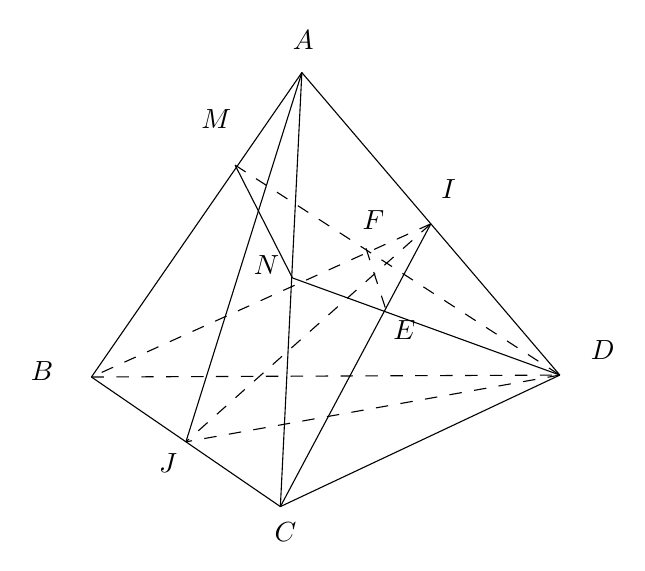
\begin{tikzpicture}[x=0.75pt,y=0.75pt,yscale=-1,xscale=1]
				%uncomment if require: \path (0,300); %set diagram left start at 0, and has height of 300
				
				%Straight Lines [id:da47172093832542683] 
				\draw  [dash pattern={on 4.5pt off 4.5pt}]  (234.65,198.26) -- (460.31,197.32) ;
				%Straight Lines [id:da26093450664971973] 
				\draw    (234.65,198.26) -- (325.67,260.69) ;
				%Straight Lines [id:da9080950852780671] 
				\draw    (460.31,197.32) -- (325.67,260.69) ;
				%Straight Lines [id:da508342626341979] 
				\draw    (336.02,51.57) -- (460.31,197.32) ;
				%Straight Lines [id:da5997859657126805] 
				\draw    (336.02,51.57) -- (325.67,260.69) ;
				%Straight Lines [id:da6156882522581331] 
				\draw    (336.02,51.57) -- (234.65,198.26) ;
				%Straight Lines [id:da2039150104142735] 
				\draw    (336.02,51.57) -- (280.16,229.48) ;
				%Straight Lines [id:da10035270371145111] 
				\draw  [dash pattern={on 4.5pt off 4.5pt}]  (460.31,197.32) -- (280.16,229.48) ;
				%Straight Lines [id:da7120080061912759] 
				\draw  [dash pattern={on 4.5pt off 4.5pt}]  (398.17,124.44) -- (280.16,229.48) ;
				%Straight Lines [id:da02570479067428555] 
				\draw    (303.87,96.17) -- (331.48,150.51) ;
				%Straight Lines [id:da3960953156043232] 
				\draw  [dash pattern={on 4.5pt off 4.5pt}]  (303.87,96.17) -- (460.31,197.32) ;
				%Straight Lines [id:da6604165430813216] 
				\draw    (460.31,197.32) -- (331.48,150.51) ;
				%Straight Lines [id:da3429779367142849] 
				\draw    (398.17,124.44) -- (325.67,260.69) ;
				%Straight Lines [id:da5882500765771612] 
				\draw  [dash pattern={on 4.5pt off 4.5pt}]  (398.17,124.44) -- (234.65,198.26) ;
				%Straight Lines [id:da6870018241661464] 
				\draw  [dash pattern={on 4.5pt off 4.5pt}]  (366.93,136.24) -- (376.91,166.98) ;
				
				% Text Node
				\draw (204.19,189.74) node [anchor=north west][inner sep=0.75pt]    {$B$};
				% Text Node
				\draw (474.06,179.61) node [anchor=north west][inner sep=0.75pt]    {$D$};
				% Text Node
				\draw (321.65,266.98) node [anchor=north west][inner sep=0.75pt]    {$C$};
				% Text Node
				\draw (330.49,30.21) node [anchor=north west][inner sep=0.75pt]    {$A$};
				% Text Node
				\draw (286.35,68.21) node [anchor=north west][inner sep=0.75pt]   [align=left] {$M$};
				% Text Node
				\draw (311.62,138.6) node [anchor=north west][inner sep=0.75pt]   [align=left] {$N$};
				% Text Node
				\draw (364,117) node [anchor=north west][inner sep=0.75pt]   [align=left] {$F$};
				% Text Node
				\draw (378.91,169.98) node [anchor=north west][inner sep=0.75pt]   [align=left] {$E$};
				% Text Node
				\draw (266,234) node [anchor=north west][inner sep=0.75pt]   [align=left] {$J$};
				% Text Node
				\draw (402,102) node [anchor=north west][inner sep=0.75pt]   [align=left] {$I$};
				
				
			\end{tikzpicture}
		\end{center}
		\begin{itemchoice}
		\itemch Đúng. Ta có $ I\in AD,AD\subset (JAD)\Rightarrow I\in (JAD)\Rightarrow IJ\subset (JAD)$; $ J\in BC$,\\
		$BC\subset (IBC)\Rightarrow J\in (IBC)\Rightarrow IJ\subset (IBC)$. Vậy $ (IBC)\cap (JAD)=IJ$.
		\itemch Đúng. $ ND$ là giao tuyến của hai mặt phẳng $ (MND),(ADC)$.
		\itemch Đúng. $ BI$ là giao tuyến của hai mặt phẳng $ (BCI),(ABD)$.
		\itemch Sai. Gọi $ E=DN\cap CI$ trong $ mp(ACD)$ và $ F=DM\cap BI$ trong $ mp(ABD)$.\\
	$\heva{
		&{E\in DN,DN\subset (DMN)}\\
		&{E\in IC,IC\subset (IBC)}.
	}$\\
	$\Rightarrow E\in (DMN)\cap (IBC).\,(1)$ \\
	Tương tự: 
	$\heva{	&F\in DM,DM\subset (DMN)\\&F\in BI,BI\subset (IBC)
	.}$ \\
	$\Rightarrow F\in (DMN)\cap (IBC).$\\
	Từ $(1)$ và $(2)$ suy ra $ (DMN)\cap (IBC)=EF$.\\
	Khi đó $EF$ cắt $IJ$.
	
	\end{itemchoice}
}
\end{ex}

\begin{ex}%[1H4H1-3]
Cho bốn điểm $ A,B,C,D$ không đồng phẳng. Gọi $ M,N$ lần lượt là trung điểm của $ AC$ và $ BC$. Trên đoạn $ BD$ lấy điểm $ P$ sao cho $ BP=2PD$, $ E=CD\cap NP$. Khi đó:
	\choiceTF
	{\True $ NM$ là giao tuyến của hai mặt phẳng $\left(MNP\right)$,$ (ABC)$}
	{\True $ DC$ là giao tuyến của hai mặt phẳng $\left(BCD\right),(ADC)$}
	{\True Giao điểm của đường thẳng $ CD$ và mặt phẳng $ (MNP)$ là điểm $ E$}
	{Giao điểm của đường thẳng $ AD$ và mặt phẳng $ (MNP)$ là giao điểm của đường thẳng $ AD$ với đường thẳng $ MP$}
	\loigiai{
		\begin{center}


\tikzset{every picture/.style={line width=0.75pt}} %set default line width to 0.75pt        

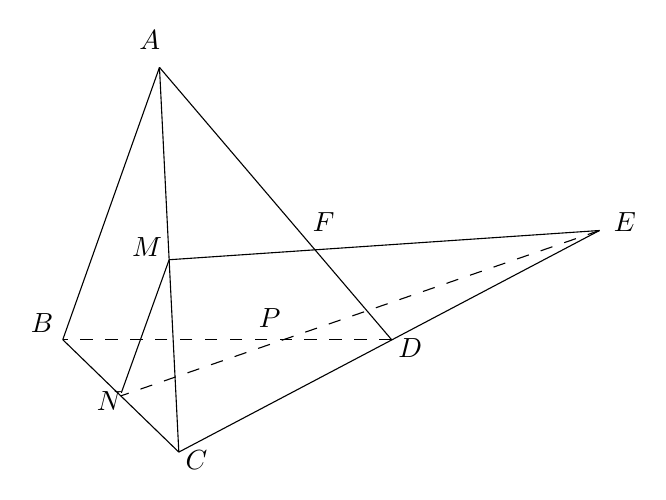
\begin{tikzpicture}[x=0.75pt,y=0.75pt,yscale=-1,xscale=1]
	%uncomment if require: \path (0,300); %set diagram left start at 0, and has height of 300
	
	%Straight Lines [id:da9292165156682857] 
	\draw  [dash pattern={on 4.5pt off 4.5pt}]  (378.21,174.4) -- (219.79,174.4) ;
	%Straight Lines [id:da9116970450235633] 
	\draw    (219.79,174.4) -- (275.7,228.57) ;
	%Straight Lines [id:da1928149712503595] 
	\draw    (266.38,43.21) -- (219.79,174.4) ;
	%Straight Lines [id:da996410268905453] 
	\draw    (266.38,43.21) -- (275.7,228.57) ;
	%Straight Lines [id:da4503117488041699] 
	\draw    (266.38,43.21) -- (378.21,174.4) ;
	%Straight Lines [id:da1440084765470453] 
	\draw    (478.38,121.8) -- (275.7,228.57) ;
	%Straight Lines [id:da36992382737671514] 
	\draw    (271.04,135.89) -- (248,200) ;
	%Straight Lines [id:da7126913576635985] 
	\draw  [dash pattern={on 4.5pt off 4.5pt}]  (478.38,121.8) -- (247.75,201.49) ;
	%Straight Lines [id:da6467375472858359] 
	\draw    (271.04,135.89) -- (478.38,121.8) ;
	
	% Text Node
	\draw (255.4,24.35) node [anchor=north west][inner sep=0.75pt]   [align=left] {$A$};
	% Text Node
	\draw (203.15,160.56) node [anchor=north west][inner sep=0.75pt]   [align=left] {$B$};
	% Text Node
	\draw (277.7,226.79) node [anchor=north west][inner sep=0.75pt]   [align=left] {$C$};
	% Text Node
	\draw (380.21,172.61) node [anchor=north west][inner sep=0.75pt]   [align=left] {$D$};
	% Text Node
	\draw (484,112) node [anchor=north west][inner sep=0.75pt]   [align=left] {$E$};
	% Text Node
	\draw (252,124) node [anchor=north west][inner sep=0.75pt]   [align=left] {$M$};
	% Text Node
	\draw (235,198) node [anchor=north west][inner sep=0.75pt]   [align=left] {$N$};
	% Text Node
	\draw (313,158) node [anchor=north west][inner sep=0.75pt]   [align=left] {$P$};
	% Text Node
	\draw (339,112) node [anchor=north west][inner sep=0.75pt]   [align=left] {$F$};
	
\end{tikzpicture}
		\end{center}
		\begin{itemchoice}
			\itemch Đúng. $NM$ là giao tuyến của hai mặt phẳng $\left(MNP\right)$,$ (ABC)$.
			\itemch Đúng. $DC$ là giao tuyến của hai mặt phẳng $\left(BCD\right),(ADC)$.
			\itemch Đúng. Tìm giao điểm của $ CD$ và mặt phẳng $ (MNP)$:\\
			Trong mặt phẳng $ (BCD)$, vì $ NP$ và $ CD$ không song song nhau nên ta có thể gọi $ E=CD\cap NP$.\\
			Trong mặt phẳng $ (BCD)$, vì $ NP$ và $ CD$ không song song nhau nên ta có thể gọi $ E=CD\cap NP$.\\
			Vì $\heva{
					&{E\in CD}\\
					&{E\in NP,NP\subset (MNP).}
				}$ \\
			$\Rightarrow E=CD\cap (MNP)$.
			\itemch Sai. Tìm giao điểm của $ AD$ và $ (MNP)$ :\\
			Xét mặt phẳng phụ là $ (ACD)$ chứa $ AD$. Ta cần tìm giao tuyến của hai mặt phẳng $ (ACD)$ và $ (MNP)$.\\
			Vì $ M\in AC,AC\subset (ACD)\Rightarrow M\in (ACD)\Rightarrow M\in (ACD)\cap (MNP).\quad(1)$\\
			Theo câu a), ta có $\heva{
					&{E\in CD,CD\subset (ACD)}\\
					&{E\in (MNP).}
			}$ \\
			$\Rightarrow E\in (ACD)\cap (MNP).\quad(2)$\\
			Từ $(1)$ và $(2)$ suy ra $ ME=(ACD)\cap (MNP)$.\\
			Trong mặt phẳng $ (ACD)$, gọi $ F=AD\cap ME$.\\
			Vì $\heva{
					&{F\in AD}\\
					&{F\in ME,ME\subset (MNP).}}$
		\end{itemchoice}
	}
\end{ex}

\begin{ex}%[1H4H1-3]
Cho tứ giác $ ABCD$ có $ AC$ và $ BD$ giao nhau tại $ O$ và một điểm $ S$ không thuộc mặt phẳng $ (ABCD)$. Trên đoạn $ SC$ lấy một điểm $ M$ không trùng với $ S$ và $ C$,$ K=AM\cap SO$. Khi đó:
	\choiceTF
	{$ SO$ là giao tuyến của hai mặt phẳng $\left(SAC\right)$,$ (ABC)$}
	{\True $ SO$ là giao tuyến của hai mặt phẳng $\left(SAC\right)$,$ (SBD)$}
	{\True Giao điểm của đường thẳng $ SO$ với mặt phẳng $ (ABM)$ là điểm $ K$}
	{Giao điểm của đường thẳng $ SD$ với mặt phẳng $ (ABM)$ là điểm $ N$ thuộc đường thẳng $ AK$}
	\loigiai{
		\begin{itemchoice}
			\itemch Sai. $ AC$ là giao tuyến của hai mặt phẳng $\left(SAC\right)$,$ (ABC)$. 
			\itemch Đúng. $SO$ là giao tuyến của hai mặt phẳng $\left(SAC\right)$,$ (SBD)$.
			\itemch Đúng. Tìm giao điểm của $ SO$ và $ (ABM)$ :\\
			Trong mặt phẳng $ (SAC)$, gọi $ K=AM\cap SO$.\\
			$\heva{
					&{K\in AM,AM\subset (ABM)}\\
					&{K\in SO}}
			\Rightarrow K=SO\cap (ABM).$\\
		\begin{center}
			
			
			\tikzset{every picture/.style={line width=0.75pt}} %set default line width to 0.75pt        
			
			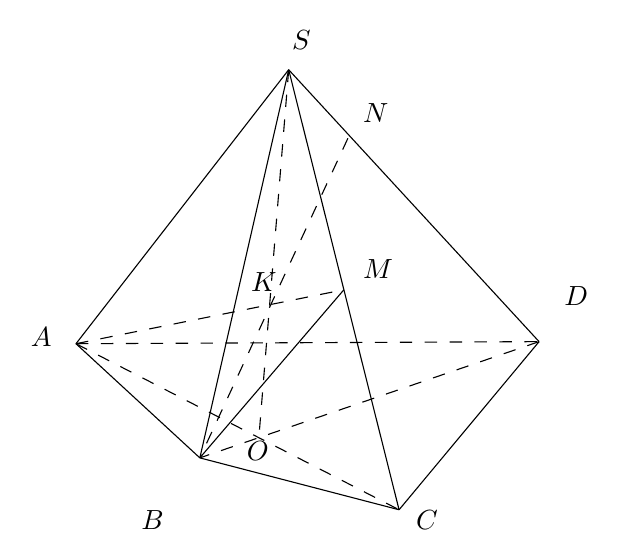
\begin{tikzpicture}[x=0.75pt,y=0.75pt,yscale=-1,xscale=1]
				%uncomment if require: \path (0,300); %set diagram left start at 0, and has height of 300
				
				%Straight Lines [id:da45140842015116234] 
				\draw [color={rgb, 255:red, 0; green, 0; blue, 0 }  ,draw opacity=1 ] [dash pattern={on 4.5pt off 4.5pt}]  (157.94,176) -- (381.06,175) ;
				%Straight Lines [id:da7826073026735398] 
				\draw [color={rgb, 255:red, 0; green, 0; blue, 0 }  ,draw opacity=1 ]   (157.94,176) -- (217.61,231) ;
				%Straight Lines [id:da9534674062185649] 
				\draw [color={rgb, 255:red, 0; green, 0; blue, 0 }  ,draw opacity=1 ]   (381.06,175) -- (313.6,256) ;
				%Straight Lines [id:da5457329414707186] 
				\draw [color={rgb, 255:red, 0; green, 0; blue, 0 }  ,draw opacity=1 ]   (217.61,231) -- (313.6,256) ;
				%Straight Lines [id:da45161295507477983] 
				\draw [color={rgb, 255:red, 0; green, 0; blue, 0 }  ,draw opacity=1 ]   (260.42,44) -- (157.94,176) ;
				%Straight Lines [id:da16147301415907722] 
				\draw [color={rgb, 255:red, 0; green, 0; blue, 0 }  ,draw opacity=1 ]   (260.42,44) -- (217.61,231) ;
				%Straight Lines [id:da35693419057228093] 
				\draw [color={rgb, 255:red, 0; green, 0; blue, 0 }  ,draw opacity=1 ]   (260.42,44) -- (313.6,256) ;
				%Straight Lines [id:da03208821732657685] 
				\draw [color={rgb, 255:red, 0; green, 0; blue, 0 }  ,draw opacity=1 ]   (260.42,44) -- (381.06,175) ;
				%Straight Lines [id:da7277007096433057] 
				\draw  [dash pattern={on 4.5pt off 4.5pt}]  (381.06,175) -- (217.61,231) ;
				%Straight Lines [id:da981556623278129] 
				\draw  [dash pattern={on 4.5pt off 4.5pt}]  (157.94,176) -- (313.6,256) ;
				%Straight Lines [id:da754666188092012] 
				\draw  [dash pattern={on 4.5pt off 4.5pt}]  (260.42,44) -- (246.15,220) ;
				%Straight Lines [id:da8695321075772138] 
				\draw  [dash pattern={on 4.5pt off 4.5pt}]  (157.94,176) -- (287.01,150) ;
				%Straight Lines [id:da8122125252711012] 
				\draw  [dash pattern={on 4.5pt off 4.5pt}]  (288.96,77) -- (217.61,231) ;
				%Straight Lines [id:da21176040951761155] 
				\draw    (287.01,150) -- (217.61,231) ;
				
				% Text Node
				\draw (260.76,24) node [anchor=north west][inner sep=0.75pt]   [align=left] {$S$};
				% Text Node
				\draw (134.93,167) node [anchor=north west][inner sep=0.75pt]   [align=left] {$A$};
				% Text Node
				\draw (391.92,147) node [anchor=north west][inner sep=0.75pt]   [align=left] {$D$};
				% Text Node
				\draw (188.12,255) node [anchor=north west][inner sep=0.75pt]   [align=left] {$B$};
				% Text Node
				\draw (320.58,255) node [anchor=north west][inner sep=0.75pt]   [align=left] {$C$};
				% Text Node
				\draw (295,59) node [anchor=north west][inner sep=0.75pt]   [align=left] {$N$};
				% Text Node
				\draw (295,134) node [anchor=north west][inner sep=0.75pt]   [align=left] {$M$};
				% Text Node
				\draw (241.02,140.5) node [anchor=north west][inner sep=0.75pt]   [align=left] {$K$};
				% Text Node
				\draw (239,222) node [anchor=north west][inner sep=0.75pt]   [align=left] {$O$};
				
				
			\end{tikzpicture}
		\end{center}
			\itemch Sai. Tìm giao điểm của $SD$ và $ (ABM)$:\\
			Xét mặt phẳng phụ $ (SBD)$ chứa $SD$.\\
			Dễ thấy $B$ là điểm chung của hai mặt phẳng $(SBD)$ và $ (ABM)$.\\
			Ta có $\heva{
					&{K\in AM,AM\subset (ABM)}\\
					&{K\in SO,SO\subset (SBD).}
			}$ \\
			$\Rightarrow K\in (SBD)\cap (ABM)$.\\
			Do đó $ BK=(SBD)\cap (ABM)$.\\
			Trong mặt phẳng $ (SBD)$, gọi $ N=BK\cap SD$.\\
		Vì $\heva{
					&{N\in SD}\\
					&{N\in BK,BK\subset (ABM)}
	           }\Rightarrow N=SD\cap (ABM).$\\
		\end{itemchoice}
	}
\end{ex}
\Closesolutionfile{ans}
\indapan{3}{ans/ans-0-B1-DS}

\Opensolutionfile{ans}[ans/ans-0-B1-KQ]
\caukq
\begin{ex}%[1H4V1-6]
	Cho tứ diện $ SABC$. Trên $ SA,SB$ và $ SC$ lần lượt lấy các điểm $ D,E$ và $ F$ sao cho $ DE$ cắt $ AB$ tại $ I,EF$ cắt $ BC$ tại $ J,DF$ cắt $ AC$ tại $ K$. Hỏi ba điểm $ I,J,K$ ở vị trí như thế nào với nhau, nếu thẳng hàng chọn $1$, không thẳng hàng chọn $2$, đồng quy chọn $3$, không nằm ở trường hợp nào của các lựa chọn trước thì chọn $4$.\\
	\shortans{$1$}
	\loigiai{
	Ta chứng minh ba điểm $ I,J,K$ đều là điểm chung của hai mặt phẳng $ (DEF)$ và $ (ABC)$.\\
\begin{center}
	
	
	\tikzset{every picture/.style={line width=0.75pt}} %set default line width to 0.75pt        
	
	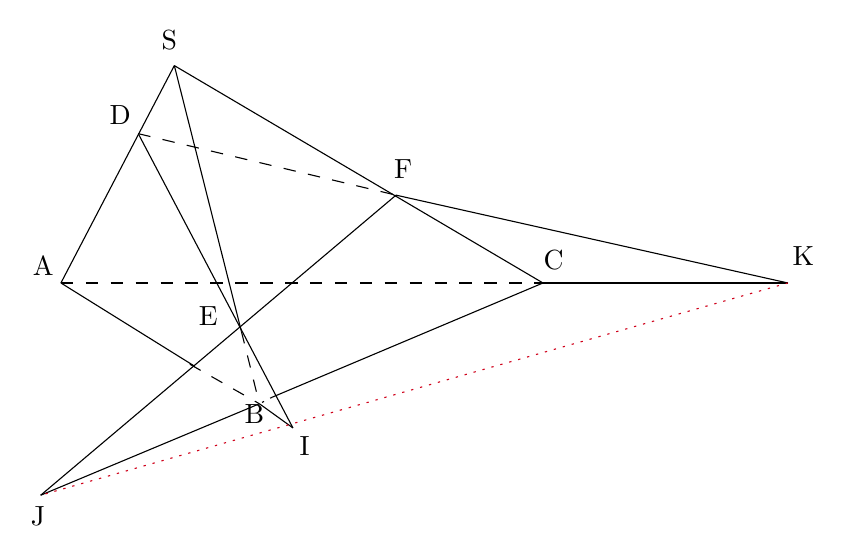
\begin{tikzpicture}[x=0.75pt,y=0.75pt,yscale=-1,xscale=1]
		%uncomment if require: \path (0,300); %set diagram left start at 0, and has height of 300
		
		%Straight Lines [id:da5842995150234604] 
		\draw  [dash pattern={on 4.5pt off 4.5pt}]  (183.75,137.74) -- (416.01,137.74) ;
		%Straight Lines [id:da39244663623132503] 
		\draw    (285.59,192.75) -- (416.01,137.74) ;
		%Straight Lines [id:da8379812814148462] 
		\draw    (183.75,137.74) -- (248.33,177.94) ;
		%Straight Lines [id:da4418001796887563] 
		\draw    (238.39,33) -- (270.69,161.01) ;
		%Straight Lines [id:da63106834651132] 
		\draw    (238.39,33) -- (183.75,137.74) ;
		%Straight Lines [id:da14302161499050037] 
		\draw    (238.39,33) -- (416.01,137.74) ;
		%Straight Lines [id:da726464341324875] 
		\draw  [dash pattern={on 4.5pt off 4.5pt}]  (221.01,65.8) -- (345.21,95.42) ;
		%Straight Lines [id:da49230277423963287] 
		\draw    (345.21,95.42) -- (534,137.74) ;
		%Straight Lines [id:da9328172858597841] 
		\draw    (416.01,137.74) -- (534,137.74) ;
		%Straight Lines [id:da7162061644965632] 
		\draw    (345.21,95.42) -- (174,240) ;
		%Straight Lines [id:da6140518997742233] 
		\draw    (221.01,65.8) -- (295.53,207.57) ;
		%Straight Lines [id:da7066750192309337] 
		\draw  [dash pattern={on 4.5pt off 4.5pt}]  (245.85,176.88) -- (279.38,195.93) ;
		%Straight Lines [id:da6653131860949277] 
		\draw    (279.38,195.93) -- (174,240) ;
		%Straight Lines [id:da34540585742962926] 
		\draw  [dash pattern={on 4.5pt off 4.5pt}]  (270.69,161.01) -- (279.38,195.93) ;
		%Straight Lines [id:da4873339161155761] 
		\draw    (295.53,207.57) -- (279.38,195.93) ;
		%Straight Lines [id:da49548564085187596] 
		\draw  [dash pattern={on 0.84pt off 2.51pt}]  (285.59,192.75) -- (279.38,195.93) ;
		%Straight Lines [id:da12662542861183668] 
		\draw [color={rgb, 255:red, 208; green, 2; blue, 27 }  ,draw opacity=1 ] [dash pattern={on 0.84pt off 2.51pt}]  (534,137.74) -- (174,240) ;
		
		% Text Node
		\draw (231,15) node [anchor=north west][inner sep=0.75pt]   [align=left] {S};
		% Text Node
		\draw (169,124) node [anchor=north west][inner sep=0.75pt]   [align=left] {A};
		% Text Node
		\draw (271,195) node [anchor=north west][inner sep=0.75pt]   [align=left] {B};
		% Text Node
		\draw (249,148) node [anchor=north west][inner sep=0.75pt]   [align=left] {E};
		% Text Node
		\draw (343,77) node [anchor=north west][inner sep=0.75pt]   [align=left] {F};
		% Text Node
		\draw (535,119) node [anchor=north west][inner sep=0.75pt]   [align=left] {K};
		% Text Node
		\draw (297.53,210.57) node [anchor=north west][inner sep=0.75pt]   [align=left] {I};
		% Text Node
		\draw (168,244) node [anchor=north west][inner sep=0.75pt]   [align=left] {J};
		% Text Node
		\draw (206,51) node [anchor=north west][inner sep=0.75pt]   [align=left] {D};
		% Text Node
		\draw (415,121) node [anchor=north west][inner sep=0.75pt]   [align=left] {C};
		
		
	\end{tikzpicture}
\end{center}
	Ta có $\heva{
			{I\in DE,DE\subset (DEF)}\\
			{I\in AB,AB\subset (ABC).}
		}$ \\
		$\Rightarrow I\in (DEF)\cap (ABC).\,(1)$\\
	Tương tự, ta có $\heva{
			&{J\in EF,EF\subset (DEF)}\\
			&{J\in BC,BC\subset (ABC).}
		}$\\
		$\Rightarrow J\in (DEF)\cap (ABC).\,(2)$\\
 	$\heva{
			&{K\in DF,DF\subset (DEF)}\\
			&{K\in AC,AC\subset (ABC).}
		}$ \\$\Rightarrow K\in (DEF)\cap (ABC).\, (3)$\\
	Từ $(1)$, $(2)$, $(3)$ suy ra $ I,J,K$ cùng thuộc hai mặt phẳng $ (DEF),(ABC)$.\\
	Vì vậy ba điểm $ I,J,K$ thẳng hàng.}
\end{ex}

\begin{ex}%[1H4V1-6]
	Cho tứ diện $ ABCD$. Gọi $ E,F,G$ là các điểm lần lượt thuộc các cạnh $ AB,AC,BD$ sao cho $ EF$ cắt $ BC$ tại $ I,EG$ cắt $ AD$ tại $ H$. Nếu ba đường thẳng $ CD,IG,HF$ đồng quy thì chọn $1$, không đồng quy thì chọn $2$, song song thì chọn $3$, chéo nhau thì chọn $4$, không nằm ở trường hợp nào của các lựa chọn trước thì chọn $5$.
	\loigiai{
		\begin{center}
			
			
			\tikzset{every picture/.style={line width=0.75pt}} %set default line width to 0.75pt        
			
			\begin{tikzpicture}[x=0.75pt,y=0.75pt,yscale=-1,xscale=1]
				%uncomment if require: \path (0,316); %set diagram left start at 0, and has height of 316
				
				%Straight Lines [id:da13687667734107634] 
				\draw  [dash pattern={on 4.5pt off 4.5pt}]  (183.75,137.74) -- (538,138) ;
				%Straight Lines [id:da08166931944525158] 
				\draw  [dash pattern={on 4.5pt off 4.5pt}]  (347.69,166.83) -- (416.01,137.74) ;
				%Straight Lines [id:da23227629868514188] 
				\draw    (183.75,137.74) -- (279.38,195.93) ;
				%Straight Lines [id:da0037299028542367996] 
				\draw    (238.39,33) -- (304,294) ;
				%Straight Lines [id:da6501354714516638] 
				\draw    (238.39,33) -- (183.75,137.74) ;
				%Straight Lines [id:da6548503643118921] 
				\draw    (238.39,33) -- (364,106) ;
				%Straight Lines [id:da8094547223274555] 
				\draw    (216,74) -- (304,294) ;
				%Straight Lines [id:da06048037959235808] 
				\draw    (364,106) -- (304,294) ;
				%Straight Lines [id:da80682584904723] 
				\draw  [dash pattern={on 4.5pt off 4.5pt}]  (216,74) -- (364,106) ;
				%Straight Lines [id:da11962693568483673] 
				\draw  [dash pattern={on 4.5pt off 4.5pt}]  (260,184) -- (347.69,166.83) ;
				%Straight Lines [id:da4410724764669989] 
				\draw    (347.69,166.83) -- (538,138) ;
				%Straight Lines [id:da30065783831976156] 
				\draw    (364,106) -- (538,138) ;
				%Straight Lines [id:da42540954354317173] 
				\draw  [dash pattern={on 4.5pt off 4.5pt}]  (364,106) -- (416.01,137.74) ;
				%Straight Lines [id:da08283497424657837] 
				\draw    (342,168) -- (279.38,195.93) ;
				
				% Text Node
				\draw (541,124) node [anchor=north west][inner sep=0.75pt]   [align=left] {I};
				% Text Node
				\draw (235,13) node [anchor=north west][inner sep=0.75pt]   [align=left] {A};
				% Text Node
				\draw (167,130) node [anchor=north west][inner sep=0.75pt]   [align=left] {B};
				% Text Node
				\draw (205,61) node [anchor=north west][inner sep=0.75pt]   [align=left] {E};
				% Text Node
				\draw (361,90) node [anchor=north west][inner sep=0.75pt]   [align=left] {F};
				% Text Node
				\draw (286,197) node [anchor=north west][inner sep=0.75pt]   [align=left] {D};
				% Text Node
				\draw (414,120) node [anchor=north west][inner sep=0.75pt]   [align=left] {C};
				% Text Node
				\draw (282,288) node [anchor=north west][inner sep=0.75pt]   [align=left] {H};
				% Text Node
				\draw (344,171) node [anchor=north west][inner sep=0.75pt]   [align=left] {O};
				% Text Node
				\draw (245,185) node [anchor=north west][inner sep=0.75pt]   [align=left] {G};
				
				
			\end{tikzpicture}
		\end{center}
		
	Trong mặt phẳng $ (BCD)$, gọi $ O=CD\cap IG$.\\
	Ta có $\heva{
			&{O\in IG,IG\subset (EFH)}\\
			&{O\in CD,CD\subset (ACD)}
	}$ \\
	$\Rightarrow O\in (EFH)\cap (ACD).\,(1)$\\
	Mặt khác: $ H\in AD,AD\subset (ACD)\Rightarrow H\in (ACD)\Rightarrow H\in (ACD)\cap (EFH)$.\\
	Tương tự: $ F\in AC,AC\subset (ACD)\Rightarrow F\in (ACD)\Rightarrow F\in (ACD)\cap (EFH)$.\\
	Vì vậy $ HF=(ACD)\cap (EFH).\, (2)$\\
	Từ $(1)$ và $(2)$ suy ra $O$ thuộc $ HF$ hay $ CD,IG,HF$ đồng quy tại $ O$.\\
}
\end{ex}

\begin{ex}%[1H4V2-3]
Cho tứ diện $ ABCD$ và $ M$ là một điểm bên trong $\triangle ABC,N$ là điểm bên trong của $\triangle ACD$. Gọi $ E=AM\cap BC$; $ F=AN\cap CD$ và $ G=DN\cap AC$.\\
a) đường thẳng $a$ là giao tuyến của $ (AMN)$ và $ (BCD)$\\
b) đường thẳng $b$ là giao tuyến của $ (DMN)$ và $ (ABC)$.\\
nếu $a$ và $b$ đồng phẳng thì chọn $0$, trùng nhau chọn $1$, chéo nhau chọn $2$, không nằm ở trường hợp nào của các lựa chọn trước thì chọn $3$.
	\shortans{$2$}
	\loigiai{
a) Tìm giao tuyến của $ (AMN)$ và $ (BCD)$ :\\
Trong mặt phẳng $ (ABC)$, gọi $ E=AM\cap BC$;\\
Trong mặt phẳng $ (ACD)$, gọi $ F=AN\cap CD$.\\
Ta có $\heva{
		{E\in AM,AM\subset (AMN)}\\
		{E\in BC,BC\in (BCD)}
	}$\\
	$\Rightarrow E\in (AMN)\cap (BCD).\quad(1)$\\
Tương tư$\heva{
		{F\in AN,AN\subset (AMN)}\\
		{F\in CD,CD\in (BCD).}
    }$\\
    $\Rightarrow F\in (AMN)\cap (BCD).\quad (2)$\\
Từ $(1)$ và $(2)$ suy ra $ EF=(AMN)\cap (BCD)$.
\begin{center}
	
	


\tikzset{every picture/.style={line width=0.75pt}} %set default line width to 0.75pt        

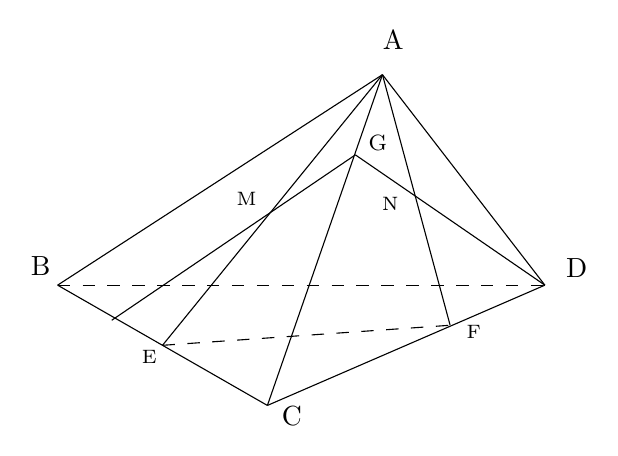
\begin{tikzpicture}[x=0.75pt,y=0.75pt,yscale=-1,xscale=1]
	%uncomment if require: \path (0,300); %set diagram left start at 0, and has height of 300
	
	%Straight Lines [id:da10666062974247015] 
	\draw  [dash pattern={on 4.5pt off 4.5pt}]  (108.04,150.99) -- (342.81,150.99) ;
	%Straight Lines [id:da1898558379683537] 
	\draw    (108.04,150.99) -- (209.12,208.94) ;
	%Straight Lines [id:da1880342280317313] 
	\draw    (342.81,150.99) -- (209.12,208.94) ;
	%Straight Lines [id:da36495199433745085] 
	\draw    (108.04,150.99) -- (264.55,49.58) ;
	%Straight Lines [id:da28620675764608783] 
	\draw    (209.12,208.94) -- (264.55,49.58) ;
	%Straight Lines [id:da022973095374406283] 
	\draw    (342.81,150.99) -- (264.55,49.58) ;
	%Straight Lines [id:da16497343245909302] 
	\draw    (264.55,49.58) -- (158.58,179.97) ;
	%Straight Lines [id:da7107402826116258] 
	\draw    (264.55,49.58) -- (297.16,170.31) ;
	%Straight Lines [id:da03351864873321908] 
	\draw  [dash pattern={on 4.5pt off 4.5pt}]  (158.58,179.97) -- (297.16,170.31) ;
	%Straight Lines [id:da860333298039528] 
	\draw    (342.81,150.99) -- (251.51,88.21) ;
	%Straight Lines [id:da31892997517062893] 
	\draw    (251.51,88.21) -- (134.13,167.9) ;
	
	% Text Node
	\draw (263.45,27.2) node [anchor=north west][inner sep=0.75pt]   [align=left] {A};
	% Text Node
	\draw (256.61,77.49) node [anchor=north west][inner sep=0.75pt]  [font=\footnotesize] [align=left] {G};
	% Text Node
	\draw (214.85,208.29) node [anchor=north west][inner sep=0.75pt]   [align=left] {C};
	% Text Node
	\draw (93.89,135.85) node [anchor=north west][inner sep=0.75pt]   [align=left] {B};
	% Text Node
	\draw (351.8,137.06) node [anchor=north west][inner sep=0.75pt]   [align=left] {D};
	% Text Node
	\draw (147.38,181.11) node [anchor=north west][inner sep=0.75pt]  [font=\scriptsize] [align=left] {E};
	% Text Node
	\draw (303.89,169.04) node [anchor=north west][inner sep=0.75pt]  [font=\scriptsize] [align=left] {F};
	% Text Node
	\draw (263.13,107.46) node [anchor=north west][inner sep=0.75pt]  [font=\scriptsize] [align=left] {N};
	% Text Node
	\draw (193.03,105.05) node [anchor=north west][inner sep=0.75pt]  [font=\scriptsize] [align=left] {M};
	
	
\end{tikzpicture}
\end{center}
b) Tìm giao tuyến của $ (DMN)$ và $ (ABC)$ :\\
Ta có $ M\in AE,AE\subset (ABC)\Rightarrow M\in (ABC)\Rightarrow M\in (ABC)\cap (DMN)$.(3)\\
Trong mặt phẳng $ (ACD)$, gọi $ G=DN\cap AC$.\\
Ta có $\heva{
		{G\in AC,AC\subset (ABC)}\\
		{G\in DN,DN\subset (DMN).}
	}\Rightarrow G\in (ABC)\cap (DMN).\,(4)$\\
Từ $(3)$ và $(4)$ suy ra $ MG=(DMN)\cap (ABC)$.
	}
\end{ex}

\begin{ex}%[0D1H1-2]
Cho tứ diện $ ABCD$. Gọi $ M,N$ lần lượt là trung điểm của $ AB$ và $ CD$. Mặt phẳng $ (\alpha)$ qua $ MN$ cắt $ AD,BC$ lần lượt tại $ P$ và $ Q$. Biết $ MP$ cắt $ NQ$ tại $ I$. Hỏi ba điểm $ I,B,D$ có thẳng hàng chọn $1$, không thẳng hàng chọn $2$, trùng nhau chọn $3$, không nằm ở trường hợp nào của các lựa chọn trước thì chọn $4$.\\
	\shortans{$1$}
\loigiai{
\begin{center}
	
	
	\tikzset{every picture/.style={line width=0.75pt}} %set default line width to 0.75pt        
	
	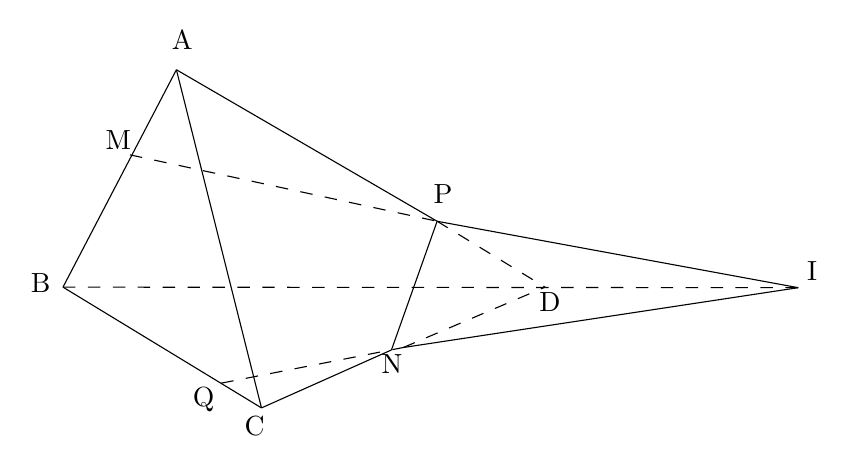
\begin{tikzpicture}[x=0.75pt,y=0.75pt,yscale=-1,xscale=1]
		%uncomment if require: \path (0,316); %set diagram left start at 0, and has height of 316
		
		%Straight Lines [id:da6286201206018192] 
		\draw  [dash pattern={on 4.5pt off 4.5pt}]  (183.75,137.74) -- (538,138) ;
		%Straight Lines [id:da10947049082539295] 
		\draw  [dash pattern={on 4.5pt off 4.5pt}]  (347.69,166.83) -- (416.01,137.74) ;
		%Straight Lines [id:da6439998262613915] 
		\draw    (183.75,137.74) -- (279.38,195.93) ;
		%Straight Lines [id:da4040708391296295] 
		\draw    (238.39,33) -- (279.38,195.93) ;
		%Straight Lines [id:da015205711258941434] 
		\draw    (238.39,33) -- (183.75,137.74) ;
		%Straight Lines [id:da7086820388098531] 
		\draw    (238.39,33) -- (364,106) ;
		%Straight Lines [id:da7046520317035536] 
		\draw    (364,106) -- (342,168) ;
		%Straight Lines [id:da3247816925100908] 
		\draw  [dash pattern={on 4.5pt off 4.5pt}]  (216,74) -- (364,106) ;
		%Straight Lines [id:da2982223830636681] 
		\draw  [dash pattern={on 4.5pt off 4.5pt}]  (260,184) -- (347.69,166.83) ;
		%Straight Lines [id:da14873030476080418] 
		\draw    (347.69,166.83) -- (538,138) ;
		%Straight Lines [id:da9330284020720327] 
		\draw    (364,106) -- (538,138) ;
		%Straight Lines [id:da44066032395990584] 
		\draw  [dash pattern={on 4.5pt off 4.5pt}]  (364,106) -- (416.01,137.74) ;
		%Straight Lines [id:da6792159322444109] 
		\draw    (342,168) -- (279.38,195.93) ;
		
		% Text Node
		\draw (541,124) node [anchor=north west][inner sep=0.75pt]   [align=left] {I};
		% Text Node
		\draw (235,13) node [anchor=north west][inner sep=0.75pt]   [align=left] {A};
		% Text Node
		\draw (167,130) node [anchor=north west][inner sep=0.75pt]   [align=left] {B};
		% Text Node
		\draw (203,61) node [anchor=north west][inner sep=0.75pt]   [align=left] {M};
		% Text Node
		\draw (361,87) node [anchor=north west][inner sep=0.75pt]   [align=left] {P};
		% Text Node
		\draw (412,139) node [anchor=north west][inner sep=0.75pt]   [align=left] {D};
		% Text Node
		\draw (270,199) node [anchor=north west][inner sep=0.75pt]   [align=left] {C};
		% Text Node
		\draw (336,169) node [anchor=north west][inner sep=0.75pt]   [align=left] {N};
		% Text Node
		\draw (245,185) node [anchor=north west][inner sep=0.75pt]   [align=left] {Q};
		
	\end{tikzpicture}
\end{center}
Ta có: $ (ABD)\cap (BCD)=BD$.\\
Mặt khác: $\heva{
		{I\in MP,MP\subset (ABD)}\\
		{I\in NQ,NQ\subset (BCD)}
	}$\\
	$\Rightarrow I\in (ABD)\cap (BCD)$.\\
Do đó $ I$ thuộc giao tuyến của hai mặt phẳng $ (ABD)$ và $ (BCD)$ hay $ I\in BD$.\\
Vậy ba điểm $ I,B,D$ thẳng hàng.}
\end{ex}

\begin{ex}%[1H4H1-6]
Cho hình chóp tứ giác $ S.ABCD$, gọi $ O$ là giao điểm của hai đường chéo $ AC$ và $ BD$. Một mặt phẳng $ (\alpha)$ cắt các cạnh bên $ SA,SB,SC,SD$ tương ứng tại các điểm $ M,N,P,Q$. Nếu các đường thẳng $ MP,NQ,SO$ nếu có đồng quy chọn $1$ không đồng quy chọn $2$, trùng nhau chọn $3$, song song đôi một chọn $3$ không nằm ở trường hợp nào của các lựa chọn trước thì chọn $4$.
	\shortans{$1$}
\loigiai{
\begin{center}
	
	
	\tikzset{every picture/.style={line width=0.75pt}} %set default line width to 0.75pt        
	
	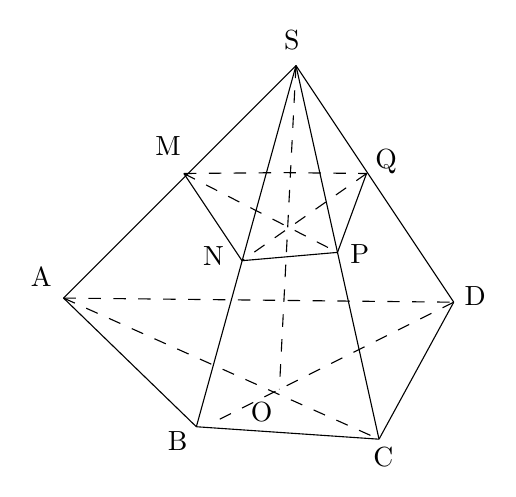
\begin{tikzpicture}[x=0.75pt,y=0.75pt,yscale=-1,xscale=1]
		%uncomment if require: \path (0,300); %set diagram left start at 0, and has height of 300
		
		%Straight Lines [id:da9649920181235869] 
		\draw  [dash pattern={on 4.5pt off 4.5pt}]  (140,170) -- (328,172) ;
		%Straight Lines [id:da9988463505885548] 
		\draw    (140,170) -- (204,232) ;
		%Straight Lines [id:da26945369399618313] 
		\draw    (292,238) -- (204,232) ;
		%Straight Lines [id:da6264568342588279] 
		\draw    (328,172) -- (292,238) ;
		%Straight Lines [id:da6368935226543855] 
		\draw  [dash pattern={on 4.5pt off 4.5pt}]  (140,170) -- (292,238) ;
		%Straight Lines [id:da27190433322613194] 
		\draw  [dash pattern={on 4.5pt off 4.5pt}]  (328,172) -- (212,230) ;
		%Straight Lines [id:da05819295714628292] 
		\draw  [dash pattern={on 4.5pt off 4.5pt}]  (252,58) -- (244,214) ;
		%Straight Lines [id:da01864638890161796] 
		\draw    (252,58) -- (140,170) ;
		%Straight Lines [id:da0209268668618956] 
		\draw    (252,58) -- (204,232) ;
		%Straight Lines [id:da3735731652545884] 
		\draw    (252,58) -- (328,172) ;
		%Straight Lines [id:da12073031506927245] 
		\draw    (252,58) -- (292,238) ;
		%Straight Lines [id:da5191440773395828] 
		\draw    (198,110) -- (226,152) ;
		%Straight Lines [id:da2776592118858545] 
		\draw    (286,110) -- (272,148) ;
		%Straight Lines [id:da10875339228030345] 
		\draw  [dash pattern={on 4.5pt off 4.5pt}]  (198,110) -- (245.48,109.57) -- (286,110) ;
		%Straight Lines [id:da8970900555244181] 
		\draw    (272,148) -- (226,152) ;
		%Straight Lines [id:da5916794330113988] 
		\draw  [dash pattern={on 4.5pt off 4.5pt}]  (198,110) -- (272,148) ;
		%Straight Lines [id:da8468730178506514] 
		\draw  [dash pattern={on 4.5pt off 4.5pt}]  (286,110) -- (226,152) ;
		
		% Text Node
		\draw (245,40) node [anchor=north west][inner sep=0.75pt]   [align=left] {S};
		% Text Node
		\draw (123,154) node [anchor=north west][inner sep=0.75pt]   [align=left] {A};
		% Text Node
		\draw (189,233) node [anchor=north west][inner sep=0.75pt]   [align=left] {B};
		% Text Node
		\draw (288,241) node [anchor=north west][inner sep=0.75pt]   [align=left] {C};
		% Text Node
		\draw (332,163) node [anchor=north west][inner sep=0.75pt]   [align=left] {D};
		% Text Node
		\draw (229,219) node [anchor=north west][inner sep=0.75pt]   [align=left] {O};
		% Text Node
		\draw (183,91) node [anchor=north west][inner sep=0.75pt]   [align=left] {M};
		% Text Node
		\draw (206,144) node [anchor=north west][inner sep=0.75pt]   [align=left] {N};
		% Text Node
		\draw (277,143) node [anchor=north west][inner sep=0.75pt]   [align=left] {P};
		% Text Node
		\draw (289,97) node [anchor=north west][inner sep=0.75pt]   [align=left] {Q};
		
		
	\end{tikzpicture}
\end{center}
Trong mặt phẳng $ (MNPQ)$ gọi $ I=MP\cap NQ$.\\
Ta sẽ chứng minh $ I\in SO$.\\
Dễ thấy $ S$ là điểm chung của hai mặt phẳng $ (SAC)$ và $ (SBD)$; đồng thời ta có:\\
$\heva{
	&{O\in AC,AC\subset (SAC)}\\
	&{O\in BD,BD\subset (SBD)}
	}$ \\$\Rightarrow O\in (SAC)\cap (SBD).\,$\\
Vì vậy $ SO=(SAC)\cap (SBD)$.(1)\\
Mặt khác: $\heva{
		&{I\in MP,MP\subset (SAC)}\\
		&{I\in NQ,NQ\subset (SBD).}
    }\Rightarrow I\in (SAC)\cap (SBD).\,(2)$\\
Từ $(1)$ và $(2)$ suy ra $ I\in SO$ hay các đường thẳng $ MP,NQ,SO$ đồng quy tại điểm $ I$.}
\end{ex}

\begin{ex}%[1H4H2-3]
Cho điểm $ S$ nằm ngoài mặt phẳng chứa tứ giác $ ABCD$ gọi $ O=AC\cap BD$ (không có cặp cạnh đối song song). Gọi $a$ giao tuyến của hai mặt phẳng $ (SAC)$ và $ (SBD)$, so độ dài giao tuyến cạnh $a$ và độ dài với cạnh $CD$ nếu giao tuyến dài hơn $CD$ thì chọn $1$ ngắn hơn thì chọn $2$, bằng chọn $3$, không nằm ở trường hợp nào của các lựa chọn trước thì chọn $4$.
	\shortans{$2$}
\loigiai{
Trong $ (ABCD)$, gọi $ O=AC\cap BD$.\\
Ta có
$\heva{
			&{O\in AC\subset (SAC)}\\
			&{O\in BD\subset (SBD)}}$
	$\Rightarrow O\in (SAC)\cap (SBD)$.\\
	$MS\in (SAC)\cap (SBD)$\\
	$\Rightarrow SO=(SAC)\cap (SBD)$
\begin{center}
	\tikzset{every picture/.style={line width=0.75pt}} %set default line width to 0.75pt        
	
	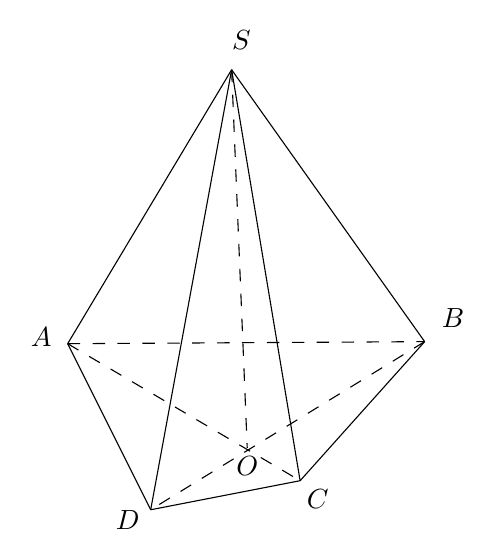
\begin{tikzpicture}[x=0.75pt,y=0.75pt,yscale=-1,xscale=1]
		%uncomment if require: \path (0,300); %set diagram left start at 0, and has height of 300
		
		%Straight Lines [id:da575608178282691] 
		\draw [color={rgb, 255:red, 0; green, 0; blue, 0 }  ,draw opacity=1 ] [dash pattern={on 4.5pt off 4.5pt}]  (152,176) -- (324,175) ;
		%Straight Lines [id:da4248466339274348] 
		\draw [color={rgb, 255:red, 0; green, 0; blue, 0 }  ,draw opacity=1 ]   (152,176) -- (192,256) ;
		%Straight Lines [id:da9556175916709888] 
		\draw [color={rgb, 255:red, 0; green, 0; blue, 0 }  ,draw opacity=1 ]   (324,175) -- (264,242) ;
		%Straight Lines [id:da45039350864708183] 
		\draw [color={rgb, 255:red, 0; green, 0; blue, 0 }  ,draw opacity=1 ]   (192,256) -- (264,242) ;
		%Straight Lines [id:da26541775038224347] 
		\draw [color={rgb, 255:red, 0; green, 0; blue, 0 }  ,draw opacity=1 ]   (231,44) -- (152,176) ;
		%Straight Lines [id:da10496555760002813] 
		\draw [color={rgb, 255:red, 0; green, 0; blue, 0 }  ,draw opacity=1 ]   (231,44) -- (192,256) ;
		%Straight Lines [id:da12955671213084963] 
		\draw [color={rgb, 255:red, 0; green, 0; blue, 0 }  ,draw opacity=1 ]   (231,44) -- (264,242) ;
		%Straight Lines [id:da28109086225514135] 
		\draw [color={rgb, 255:red, 0; green, 0; blue, 0 }  ,draw opacity=1 ]   (231,44) -- (324,175) ;
		%Straight Lines [id:da47941057692627487] 
		\draw  [dash pattern={on 4.5pt off 4.5pt}]  (152,176) -- (264,242) ;
		%Straight Lines [id:da6730001977328921] 
		\draw  [dash pattern={on 4.5pt off 4.5pt}]  (324,175) -- (192,256) ;
		%Straight Lines [id:da20811140673389716] 
		\draw  [dash pattern={on 4.5pt off 4.5pt}]  (231,44) -- (238.51,226.23) ;
		
		% Text Node
		\draw (230,24) node [anchor=north west][inner sep=0.75pt]   [align=left] {$S$};
		% Text Node
		\draw (133,167) node [anchor=north west][inner sep=0.75pt]   [align=left] {$A$};
		% Text Node
		\draw (331,158) node [anchor=north west][inner sep=0.75pt]   [align=left] {$B$};
		% Text Node
		\draw (174,255) node [anchor=north west][inner sep=0.75pt]   [align=left] {$D$};
		% Text Node
		\draw (266,245) node [anchor=north west][inner sep=0.75pt]   [align=left] {$C$};
		% Text Node
		\draw (232,229) node [anchor=north west][inner sep=0.75pt]   [align=left] {$O$};
	\end{tikzpicture}
\end{center}
}
\end{ex}
\Closesolutionfile{ans}
\indapan{6}{ans/ans-0-B1-KQ}

\subsection{Đề 2}
\Opensolutionfile{ans}[ans/ans-0-B1]
\caulc
\begin{ex}%[1H4H1-4]
	Cho hình chóp $S.ABCD$. Gọi $M$ là một điểm trên đoạn $SA$. Giao điểm của đường thẳng $CM$ với mặt phẳng $(SBD)$ là điểm nào?
	\choice
	{Điểm $ I$ với $I=CM\cap BD$}
	{\True Điểm $J$ với $J=CM\cap SO$ và $O=AC\cap BD$}
	{Điểm $H$ với $H=CM\cap SB$}
	{Điểm $N$ với $N=CM\cap SD$}
	\loigiai{
		\immini{
			Trong $\left(ABCD\right)$, gọi $ O=AC\cap BD$.\\ Suy ra $(SAC)\cap(SBD)=SO$.\\
			Trong $(SAC)$, gọi $J=CM\cap SO$.\\
			Ta có $\heva{&J\in CM\\&J\in SO,~ SO \subset (SBD)\Rightarrow J \in (SBD).} $\\
			Vậy $ J=CM\cap(SBD)$.}
		{
			\begin{tikzpicture}[scale=0.8,line join=round, font=\footnotesize, line cap=round]
				\coordinate (S) at (1,4);
				\coordinate (A) at (-2,0);
				\coordinate (B) at (0,-1.5);
				\coordinate (C) at (3,-2);
				\coordinate (D) at (5,0);
				\coordinate (M) at ($(S)!0.3!(A)$);
				\coordinate (O) at (intersection of A--C and B--D);
				\coordinate (J) at (intersection of S--O and C--M);
				\draw(S)--(A) (S)--(B) (S)--(C) (S)--(D) (B)--(C) (A)--(B)--(C)--(D);
				\draw[dashed] (C)--(A)--(D)--(B) (C)--(M) (S)--(O);
				\foreach \i/\g in {S/90,A/180,B/-90,C/-90,D/0, M/160, O/-90, J/0}{\draw[fill=black](\i) circle (1pt) ($(\i)+(\g:3mm)$) node{$\i$};}
			\end{tikzpicture}
		}
	}
\end{ex}

\begin{ex}%[1H4H1-5]
	Cho tứ diện $ABCD$ có $M$, $N$ lần lượt là trung điểm của $AB$, $CD$ và $P$ là một điểm thuộc cạnh $ BC$ ($P$ không là trung điểm của $BC$). Thiết diện của tứ diện bị cắt bởi mặt phẳng $(MNP)$ là
	\choice
	{\True Tứ giác}
	{Ngũ giác}
	{Lục giác}
	{Tam giác}
	\loigiai{
		\begin{center}
			\begin{tikzpicture}[scale=0.8, font=\footnotesize, line join=round, line cap=round]
				\coordinate (A) at (0,4);
				\coordinate (B) at (-2.5,0);
				\coordinate (C) at (1,-2.5);
				\coordinate (D) at (3,0);
				\coordinate (M) at ($(A)!0.5!(B)$);
				\coordinate (N) at ($(C)!0.5!(D)$);
				\coordinate (P) at ($(B)!0.3!(C)$);
				\coordinate (Q) at (intersection of P--N and B--D);
				\coordinate (R) at (intersection of Q--M and A--D);
				\draw (A)--(M)--(P)--(C)--(D)--(A)--(C) (P)--(Q)--(M) (R)--(N);
				\draw[dashed,thin] (Q)--(D) (P)--(B)--(M)--(N)--(P) (M)--(R);
				\foreach \i/\g in {A/90,B/-90,C/-90,D/0, P/-90, Q/-180, N/-60, M/120, R/20}{\draw[fill=black](\i) circle (1pt) ($(\i)+(\g:3mm)$) node {$\i$};}
			\end{tikzpicture}
		\end{center}
		Gọi $ Q=NP\cap BD$. Gọi $ R=QM\cap AD$. Suy ra $P$, $Q\in (MNP)$.\\
		Vậy thiết diện của tứ diện bị cắt bởi mặt phẳng $(MNP)$ là tứ giác $MRNP$.}
\end{ex}

\begin{ex}%%[1H4H3-5]
	Cắt hình chóp tứ giác bởi mặt phẳng vuông góc với đường cao của hình chóp thiết diện là hình gì?
	\choice
	{Một hình bình hành}
	{Một ngũ giác}
	{\True Một hình tứ giác}
	{Một hình tam giác}
	\loigiai{
		\begin{center}
			\begin{tikzpicture}[scale=0.8,line join=round, font=\footnotesize, line cap=round]
				\coordinate (S) at (1,4);
				\coordinate (A) at (-2,0);
				\coordinate (B) at (0,-1.5);
				\coordinate (C) at (3,-2);
				\coordinate (D) at (5,0);
				\coordinate (M) at ($(S)!0.4!(A)$);
				\coordinate (N) at ($(S)!0.4!(B)$);
				\coordinate (P) at ($(S)!0.4!(C)$);
				\coordinate (Q) at ($(S)!0.4!(D)$);
				\draw (S)--(A)--(B)--(C)--(D)--(S)--(A) (B)--(S)--(C) (M)--(N)--(P)--(Q);
				\draw[dashed] (A)--(D) (M)--(Q);
				\foreach \i/\g in {S/90,A/180,B/-90,C/-90,D/0, M/180, N/-140, P/0, Q/0}{\draw[fill=black](\i) circle (1pt) ($(\i)+(\g:3mm)$) node{$\i$};}
			\end{tikzpicture}
		\end{center}
		Mặt phẳng vuông góc với đường cao sẽ song song với đáy nên cắt hình chóp theo đa giác đồng dạng với đáy.\\
		Vậy thiết diện là hình tứ giác.}
\end{ex}

\begin{ex}%[1H4H1-3]
	Cho hình chóp $S.ABCD$ có đáy $ABCD$ là hình thang với đáy lớn $AD$. Gọi $M$ là trung điểm của $CD$. Giao tuyến của hai mặt phẳng $(MSB)$ và $(SAC)$ là đường thẳng
	\choice
	{\True $SI$ với $I$ là giao điểm của $AC$ và $BM$}
	{$SP$ với $P$ là giao điểm của $AB$ và $CD$}
	{$SI$ với $J$ là giao điểm của $AM$ và $BD$}
	{$SO$ với $O$ là giao điểm của $AC$ và $BD$}
	\loigiai{
		\immini{
			Ta có $S$ là điểm chung của hai mặt phẳng $(SAC)$ và $(SBM)$.\\
			Trong $(ABCD)$ gọi $I=AC\cap BM$.\\
			Ta có $\heva{&I\in AC,~AC\in (SAC) \Rightarrow I \in (SAC)\\ & I \in BM,~BM\in (SBM)\Rightarrow I \in (SBM).}$\\
			Suy ra, $I$ cũng là điểm chung của hai mặt phẳng $(SAC)$ và $(SBM)$.\\
			Vậy $SI$ là giao tuyến của hai mặt phẳng $(SAC)$ và $(SBM)$.
		}{
			\begin{tikzpicture}[scale=0.8, font=\footnotesize, line join=round, line cap=round]
				\coordinate (A) at (0,0);
				\coordinate (B) at (0.5,-2);
				\coordinate (C) at (3.5,-2);
				\coordinate (D) at (6,0);
				\coordinate (M) at ($(C)!0.5!(D)$);
				\coordinate (S) at (2,4);
				\coordinate (I) at (intersection of A--C and B--M);
				\draw (S)--(A)--(B)--(C)--(D)--(S)--(B) (S)--(C) (S)--(M);
				\draw[dashed,thin] (A)--(D) (B)--(M) (A)--(C) (S)--(I);
				\foreach \i/\g in {S/90,A/180,B/-90,C/-90,D/0, M/-60, I/-90}{\draw[fill=black](\i) circle (1pt) ($(\i)+(\g:3mm)$) node {$\i$};}
			\end{tikzpicture}
			
		}
	}
\end{ex}

\begin{ex}%[1H4H1-3]
	Cho hình chóp $ S.ABCD$ có đáy là hình bình hành. Gọi $M$, $N$ lần lượt là trung điểm của $AD$ và $BC$. Giao tuyến của hai mặt phẳng $(SMN)$ và $(SAC)$ là
	\choice
	{$ SD$}
	{\True $ SO$ với $O$ là tâm hình bình hành $ABCD$}
	{$SG$ với $G$ là trung điểm của $AB$}
	{$ SF$ với $F$ là trung điểm $CD$}
	\loigiai{
		\immini{
			Ta có $S$ là điểm chung của hai mặt phẳng $(SMN)$ và $(SAC)$.\\
			Gọi $O$ là tâm của hình bình hành $ABCD$ nên $AC\cap MN=O$\\
			Ta có $\heva{&O\in MN,~MN\in (SMN) \Rightarrow O \in (SMN)\\ & OI \in AC,~AC\in (SAC)\Rightarrow O \in (SAC).}$\\
			Suy ra, $O$ cũng là điểm chung của hai mặt phẳng $(SMN)$ và $(SAC)$.\\
			Vậy $SO$ là giao tuyến của hai mặt phẳng $(SMN)$ và $(SAC)$.}
		{
			\begin{tikzpicture}[scale=0.8, font=\footnotesize, line join=round, line cap=round]
				\coordinate (A) at (0,0);
				\coordinate (B) at (-2,-1.5);
				\coordinate (D) at (5,0);
				\coordinate (C) at ($(B)+(D)-(A)$);
				\coordinate (M) at ($(A)!0.5!(D)$);
				\coordinate (N) at ($(B)!0.5!(C)$);
				\coordinate (O) at ($(A)!0.5!(C)$);
				\coordinate (S) at (0,4);
				\draw(S)--(B)--(C)--(D)--(S)--(C) (S)--(N);
				\draw[dashed,thin] (B)--(A)--(D) (S)--(A) (B)--(D) (S)--(M)--(N) (A)--(C) (S)--(O);
				\foreach \i/\g in {S/90,A/160,B/-90,C/-90,D/0,M/60, N/-90, O/-90}{\draw[fill=black](\i) circle (1pt) ($(\i)+(\g:3mm)$) node {$\i$};}
			\end{tikzpicture}
		}
	}
\end{ex}
\begin{ex}%[1T4B3-5]
	Cho hình chóp tứ giác $S.ABCD$ có đáy $ABCD$ là hình bình hành và điểm $M$ thuộc cạnh $SB$, $M$ không trùng với $S$ và $B$. Mặt phẳng $(ADM)$ cắt hình chóp theo thiết diện là
	\choice
	{Tam giác}
	{\True Hình thang}
	{Hình bình hành}
	{Hình chữ nhật}
	\loigiai{
		\immini{Ta có
			$$\heva{&M\in(ADM) \cap(SBC)\\&AD \subset(ADM)\\&BC \subset(SBC)\\&AD\parallel BC
			} \Rightarrow(ADM) \cap(SBC)=Mx\parallel BC\parallel AD.$$
			Gọi $N$ là giao điểm của $Mx$ và $SC$. Khi đó $(ADM)$ cắt hình chóp theo thiết diện là tứ giác $ADNM$.\\
			Vì $MIN\parallel AD$ và $MN$ không bằng $AD$ nên $ADNM$ là hình thang.
		}{
			\begin{tikzpicture}[line join=round,line cap=round, font=\footnotesize,scale=1,>=stealth]
				\def\r{2.5}
				\path
				(0,0) coordinate (A)
				(\r,0) coordinate (B)
				(80:0.9*\r) coordinate (S)
				(230:0.6*\r) coordinate (D)		
				($(B)+(D)$) coordinate (C)
				($(S)!0.6!(B)$) coordinate (M)
				($(S)!0.6!(C)$) coordinate (N)
				;
				\draw (S)--(B)-- (C) --(D)--(S)--(C)(M)--(N)--(D);
				\draw[dashed] (S)--(A)--(D)(B)--(A)--(M);
				\foreach \x/\g in {S/90,A/170,B/0,C/-40,D/180,M/40,N/0}\fill[black] (\x) circle(1pt)+(\g:0.3)node{$\x$};	
			\end{tikzpicture}	 
		}	
	}
\end{ex}
\begin{ex}%[1H4N1-3]
	Cho tứ diện $ ABCD$ có $E$, $F$ lần lượt là trung điểm cạnh $BC$, $CD$ và $G$ là trọng tâm tam giác $ACD$. Giao tuyến của hai mặt phẳng $(ABG)$ và $(ACD)$ là đường thẳng nào dưới đây?
	\choice
	{$AE$}
	{\True $AF$}
	{$CD$}
	{$BG$}
	\loigiai{
		\immini{
			Ta có $A$, là điểm chung của hai mặt phẳng $(ABG)$ và $(ACD)$.\\
			Lại có $\heva{&F\in AG,~AG\in (ABG) \Rightarrow F \in (ABF)\\ & F \in CD,~CD\in (ACD)\Rightarrow F \in (ACD).}$\\
			Suy ra, $F$ cũng là điểm chung của hai mặt phẳng $(ABF)$ và $(ACD)$.\\
			Vậy $AF$ là giao tuyến của hai mặt phẳng $(ABF)$ và $(ACD)$.
		}{
			\begin{tikzpicture}[scale=0.8, font=\footnotesize, line join=round, line cap=round]
				\coordinate (A) at (0,4);
				\coordinate (B) at (-2.5,0);
				\coordinate (C) at (1,-2.5);
				\coordinate (D) at (3,0);
				\coordinate (E) at ($(B)!0.5!(C)$);
				\coordinate (F) at ($(C)!0.5!(D)$);
				\coordinate (G) at ($(A)!0.667!(F)$);
				\draw (A)--(B)--(C)--(D)--(A)--(C) (A)--(F);
				\draw[dashed,thin] (B)--(D) (G)--(B)--(F);
				\foreach \i/\g in {A/90,B/-180,C/-90,D/0, E/-90, F/-90, G/0 }{\draw[fill=black](\i) circle (1pt) ($(\i)+(\g:3mm)$) node {$\i$};}
			\end{tikzpicture}
		}
	}
\end{ex}

\begin{ex}%[1H4N1-3]
	Cho tứ diện $ABCD$. Gọi $M$, $N$ lần lượt là trung điểm của $AC$ và $DC$. Giao tuyến của hai mặt phẳng $(MBD)$ và $(ABN)$ là
	\choice
	{Đường thẳng $MN$}
	{Đường thẳng $AM$}
	{\True Đường thẳng $BG$ ($G$ là trọng tâm $\triangle ACD$)}
	{Đường thẳng $AH$ ($H$ là trực tâm $\triangle ACD$)}
	\loigiai{
		\immini{
			Vì $G$ là trọng tâm $\triangle ACD$ nên $G$ là giao điểm của hai trung tuyến $DM$ và $AN$ .\\
			Suy ra $G$ là điểm chung của $(MBD)$ và $(ABN)$.\\
			Lại có $B$ cũng là điểm chung của $(MBD)$ và $(ABN)$.\\
			Vậy $BG$ là giao tuyến của hai mặt phẳng $(MBD)$ và $(ABN)$.
		}{	\begin{tikzpicture}[scale=0.8, font=\footnotesize, line join=round, line cap=round]
				\coordinate (A) at (0,4);
				\coordinate (B) at (-2.5,0);
				\coordinate (C) at (1,-2.5);
				\coordinate (D) at (3,0);
				\coordinate (M) at ($(A)!0.5!(C)$);
				\coordinate (N) at ($(C)!0.5!(D)$);
				\coordinate (G) at ($(D)!0.667!(M)$);
				\draw (A)--(B)--(C)--(D)--(A)--(C) (B)--(M)--(D) (A)--(N);
				\draw[dashed,thin] (B)--(D) (B)--(N);
				\foreach \i/\g in {A/90,B/-180,C/-90,D/0, M/150,N/-70, G/50 }{\draw[fill=black](\i) circle (1pt) ($(\i)+(\g:3mm)$) node {$\i$};}
			\end{tikzpicture}
	}}
\end{ex}


\begin{ex}%[1H4H1-3]
	Cho tứ diện $ABCD$. Gọi $M$, $N$ lần lượt là trung điểm của $AC$, $CD$. Giao tuyến của hai mặt phẳng $\left(MBD\right)$ và $\left(ABN\right)$ là
	\choice
	{Đường thẳng $MN$}
	{\True Đường thẳng $BG$ ($G$ là trọng tâm tam giác $ACD$)}
	{Đường thẳng $AM$}
	{Đường thẳng $AN$ ($N$ là trực tâm tam giác $ACD$)}
	\loigiai{
		\begin{center}
			\begin{tikzpicture}[scale=1,font=\footnotesize,line join=round,line cap=round,>=stealth]
				\path 
				(-2,0) coordinate (B)
				(-1,-2) coordinate (C)
				(3,0) coordinate (D)
				($(B)+(2,3)$) coordinate (A)
				($(A)!0.5!(C)$) coordinate (M)
				($(C)!0.5!(D)$) coordinate (N)
				;
				\coordinate (G) at (intersection of A--N and D--M);
				\draw (A)--(B) (A)--(C) (A)--(D) (B)--(C)--(D) (B)--(M)--(D) (A)--(N);
				\draw [dashed] (N)--(B)--(D);
				\foreach \x/\g in {A/90,B/180,C/-90,D/0,M/150,N/-90,G/50} \draw[fill=black](\x) circle (.5pt) ($(\x)+(\g:3mm)$) node[scale=1]{$\x$};
			\end{tikzpicture}
		\end{center}
		Gọi $G$ là trọng tâm của tam giác $ACD$.\\
		Ta có 
		$\left.\begin{array}{l}
			B\in\left(BDM\right)\\
			B\in\left(ABN\right)
		\end{array}\right\}\Rightarrow B\in\left(BDM\right)\cap\left(ABN\right)$.\\
		Và 
		$\left.\begin{array}{l}
			AN\subset\left(ABN\right)\\
			DM\subset\left(BDM\right)\\
			DM\cap AN=\left\{G\right\}
		\end{array}\right\}G\in\left(BDM\right)\cap\left(ABN\right)$.\\
		Suy ra $\left(BDM\right)\cap\left(ABN\right)=BG$.
	}
\end{ex}
\begin{ex}%[1H4H1-3]
	Cho hình chóp tứ giác $S.ABCD$ có đáy là hình thang $( AD\parallel BC )$. Gọi $H$ là trung điểm $AB$. Giao tuyến của hai mặt phẳng $( SHD )$ và $( SAC )$ là
	\choice 
	{ \True $SI$ ($I$ là giao điểm của $HD$ và $AC$)} 
	{ $SK$ ($K$ là giao điểm của $AB$ và $CD$)} 
	{ $SO$ ($O$ là giao điểm của $AC$ và $BD$)} 
	{ $SA$}
	\loigiai{
		\immini{\begin{itemize}
				\item $S$ là điểm chung thứ nhất của $( SHD )$ và $( SAC )$.
				\item Gọi $I$ là giao điểm của $AC$ và $HD$ nên $I\in AC$, $I\in HD$ do đó $I$ là điểm chung thứ hai $( SHD )$ và $( SAC )$.
			\end{itemize}
			Vậy giao tuyến của hai mặt phẳng $( SHD )$ và $( SAC )$ là $SI$.}
		{\begin{tikzpicture}[scale=0.6, font=\footnotesize, line join=round, line cap=round, >=stealth]
				\def\bc{5} % cạnh BC
				\def\ba{3.5} % cạnh BA
				\def\h{5} % đường cao
				\def\gocB{100} % góc B của đáy
				\coordinate (B) at (0,0);
				\coordinate (A) at (\gocB:\ba);
				\coordinate (C) at (\bc,0);
				\coordinate (D) at ($(A)+(0:2*\bc)$);
				\coordinate (S) at ($(A)+(60:\h)$);
				\coordinate (H) at ($(A)!0.5!(B)$);
				\coordinate  (I) at	(intersection of C--A and H--D) ;
				\draw (B)--(C)--(D)--(S)--cycle (S)--(A)--(B) (H)--(S)--(C);
				\draw[dashed] (C)--(A)--(D) (D)--(H) (S)--(I);
				\foreach \p/\i in {A/180,B/-90,D/0,C/-90,S/90,I/-90,H/180}
				\fill (\p) circle (1.5pt) node[shift={(\i:3mm)}]{$\p$};
\end{tikzpicture}}} \end{ex} 

\begin{ex}%[1H4H1-5]
	Cho tứ diện đều $ABCD$ cạnh $a$, gọi $G$ là trọng tâm tam giác $AB$ cắt tứ diện bởi mặt phẳng $(GCD)$ được thiết diện có diện tích là:
	\choice
	{$\dfrac{a^2\sqrt 3}{4}$}
	{$\dfrac{a^2\sqrt 2}{2}$}
	{$\dfrac{a^2\sqrt 2}{6}$}
	{\True $\dfrac{a^2\sqrt 2}{4}$}
	\loigiai{
		\begin{center}
			\begin{tikzpicture}[scale=1,font=\footnotesize,line join=round,line cap=round,>=stealth]
				\path 
				(-2,0) coordinate (D)
				(-1,-2.5) coordinate (C)
				(3,0) coordinate (B)
				($(B)!0.5!(C)$) coordinate (N)
				($(D)!2/3!(N)$) coordinate (O)
				($(O)+(0,5)$) coordinate (A)
				($(A)!0.5!(B)$) coordinate (M)
				;
				\coordinate (G) at (intersection of A--N and C--M);
				\draw (A)--(B) (A)--(C) (A)--(D) (A)--(N) (M)--(C)
				(B)--(C)--(D);
				\draw[dashed] (B)--(D) (D)--(N) (A)--(O) (D)--(M);
				\foreach \x/\g in {A/90,B/0,C/-90,D/180,O/30,M/30,G/0} \draw[fill=black](\x) circle (.5pt) ($(\x)+(\g:3mm)$) node[scale=1]{$\x$};
			\end{tikzpicture}
		\end{center}
		Gọi $M$ là trung điểm của $AB$.\\
		Khi đó thiết diện cắt bởi $(GCD)$ là tam giác $CDM$.\\ 
		Ta có $\triangle CDM$ cân tại $M$ và $MD=MC=\dfrac{a\sqrt{3}}{2}$; $CD=a$.\\
		Gọi $N$ là trung điểm $CD$, tính được $MN=\sqrt{\left(\dfrac{\sqrt{3}a}{2}\right)^2-\left(\dfrac{a}{2}\right)^2}=\dfrac{a\sqrt{2}}{2}$.\\ 
		Vậy $S_{\triangle CDM}=\dfrac{a^2\sqrt{2}}{4}$.
	}
\end{ex} 

\begin{ex}%[1H4H1-3]
	Cho tứ diện $ABCD$ và điểm $M$ thuộc miền trong của tam giác $ACD$. Gọi $I$ và $J$ lần lượt là hai điểm trên cạnh $BC$ và $BD$ sao cho $IJ$ không song song với $CD$. Gọi $H$, $K$ lần lượt là giao điểm cùa $IJ$ với $CD$ của $MH$ và $AC$. Giao tuyến của hai mặt phẳng $(ACD)$ và $(IJM)$ là
	\choice
	{$KI$}
	{$KJ$}
	{$MI$}
	{\True $MH$}
	\loigiai{
		\begin{center}
			\begin{tikzpicture}[scale=1,font=\footnotesize,line join=round,line cap=round,>=stealth]
				\path 
				(-2,-2) coordinate (B)
				(3,-2) coordinate (C)
				(0,-0.5) coordinate (D)
				($(D)+(85:3)$) coordinate (A)
				($(D)+(10:1.3)$) coordinate (M)
				($(B)!0.4!(C)$) coordinate (I)
				($(B)!0.8!(D)$) coordinate (J)
				($(C)!1.5!(D)$) coordinate (x)
				($(I)!1.5!(J)$) coordinate (y)
				;
				\coordinate (H) at (intersection of C--x and I--y);
				\coordinate (z) at ($(H)!1.5!(M)$);
				\coordinate (K) at (intersection of A--C and H--z);
				\draw (A)--(B) (A)--(C) (B)--(C);
				\draw[dashed] (A)--(D) (B)--(D)--(C) (I)--(H)--(K) (J)--(M)--(I);
				\foreach \x/\g in {A/90,B/180,C/-90,D/-90,M/90,I/-90,J/180,H/90,K/0} \draw[fill=black](\x) circle (.5pt) ($(\x)+(\g:3mm)$) node[scale=1]{$\x$};
			\end{tikzpicture}
		\end{center}
		Ta có điểm $M$ thuộc miền trong của tam giác $ACD$ và $H$ là giao điểm cùa $IJ$ với $CD$ nên hai mặt phẳng $(ACD)$ và $(IJM)$ có hai điểm chung $M$ và $H$ nên có giao tuyến là $MH$.
	}
\end{ex} 



\Closesolutionfile{ans}
\indapan{6}{ans/ans-0-B1}
\cauds
\Opensolutionfile{ans}[ans/ans-0-B1-DS]
\begin{ex}%[1H4H1-5]%[1H4N3-2]%[1H4H1-3]
	Cho hình chóp $S.ABCD$ có đáy $ABCD$ là hình bình hành tâm $O$, $I$ là trung điểm cạnh $SC$. Khẳng định nào sau đây {\bf SAI}?
	\choiceTF
	{$\mathrm{mp}\ (IBD)$ cắt hình chóp $S.ABCD$ theo thiết diện là một tứ giác}
	{\True $IO \parallel \mathrm{mp}\ (SAB)$}
	{\True $(IBD) \cap (SAC)=IO$}
	{\True $IO \parallel \mathrm{mp}\ (SAD)$}
	\loigiai{
		\begin{center}
			\begin{tikzpicture}[scale=0.8, font=\footnotesize,line join=round, line cap=round, >=stealth]
				\coordinate (A) at (0,0);
				\coordinate (B) at (-2,-2);
				\coordinate (D) at (5,0);
				\coordinate (C) at ($(B)+(D)-(A)$);
				\coordinate (O) at ($(A)!0.5!(C)$);
				\coordinate (S) at ($(O)+(100:5)$);
				\coordinate (I) at ($(S)!0.5!(C)$);
				\draw (S)--(B) (S)--(C) (S)--(D)
				(B)--(C)--(D) (B)--(I)--(D);
				\draw[dashed] (S)--(A) (D)--(A)--(B)
				(A)--(C) (B)--(D) (O)--(I);
				\foreach \i/\g in {S/90,A/160,B/-90,C/-90,D/-90,O/-90,I/50}{\draw[fill=black](\i) circle (.5pt) ($(\i)+(\g:4mm)$) node[scale=1]{$\i$};}
			\end{tikzpicture}
		\end{center}
		\begin{itemchoice}
			\itemch Sai. $\left(IBD\right)$ cắt hình chóp theo thiết diện là tam giác $IBD$.
			\itemch Đúng. 
			$\left.\begin{array}{l}
				OI \parallel SA\\
				OI \not\subset (SAB)
			\end{array}\right\}
			\Rightarrow OI{\parallel}\left(SAB\right)$
			\itemch Đúng. $\left(IBD\right)\cap\left(SAC\right)=IO$.
			\itemch Đúng. 
			$\left.\begin{array}{l}
				OI \parallel SA\\
				OI \not\subset (SAD)
			\end{array}\right\}
			\Rightarrow OI{\parallel}\left(SAD\right)$.
		\end{itemchoice}
	}
\end{ex}

\begin{ex}%[1H4H1-3]%[1H4H1-4]
	Cho hình bình hành $ABCD$ và một điểm $S$ không thuộc mặt phẳng $(ABCD)$, các điểm $M, N$ lần lượt là trung điểm của đoạn thẳng $AB, SC$. Gọi $O=AC\cap BD$.
	\choiceTF
	{\True $SO$ giao tuyến của hai mặt phẳng $(SAC)$ và $(SBD)$}
	{\True Giao điểm của $I$ của đường thẳng $AN$ và mặt phẳng $(SBD)$ là điểm nằm trên đường thẳng $SO$}
	{Giao điểm của $J$ của đường thẳng $MN$ và mặt phẳng $(SBD)$ là điểm nằm trên đường thẳng $SD$}
	{\True Ba điểm $I, J, B$ thẳng hàng}
	\loigiai{
		\begin{center}
			\begin{tikzpicture}[scale=0.8, font=\footnotesize,line join=round, line cap=round, >=stealth]
				\coordinate (A) at (0,0);
				\coordinate (B) at (2,-2);
				\coordinate (D) at (5,0);
				\coordinate (C) at ($(B)+(D)-(A)$);
				\coordinate (S) at ($(A)+(50:6)$);
				\coordinate (N) at ($(S)!0.5!(C)$);
				\coordinate (M) at ($(A)!0.5!(B)$);
				\coordinate (O) at (intersection of A--C and B--D);
				\coordinate (I) at (intersection of A--N and S--O);
				\coordinate (P) at (intersection of C--M and B--D);
				\coordinate (J) at (intersection of S--P and M--N);
				\draw (S)--(A) (S)--(B) (S)--(C) (A)--(B)--(C);
				\draw[dashed] (S)--(D) (S)--(O) (A)--(D)--(C) (A)--(C) (B)--(D) (M)--(N)--(A) (S)--(P) (C)--(M);
				\foreach \i/\g in {S/90,A/180,B/-90,C/-90,D/0,M/180,N/0,I/60,J/160,P/-90,O/0}{\draw[fill=black](\i) circle (.5pt) ($(\i)+(\g:3mm)$) node[scale=1]{$\i$};}
			\end{tikzpicture}
		\end{center}
		\begin{itemchoice}
			\itemch Đúng. $SO$ giao tuyến của hai mặt phẳng $(SAC)$ và $(SBD)$.
			\itemch Đúng.
			Trong mặt phẳng $(ABCD)$, gọi $O=AC\cap BD$.\\
			Trong mặt phẳng $(SAC)$, gọi $I=SO\cap AN$.\\
			Ta có
			$\heva{
				& I\in AN\\
				& I\in SO, SO\subset (SBD)
			}
			\Rightarrow I=AN\cap (SBD)$.
			\itemch Sai. Tìm giao điểm $J$ của $MN$ và mặt phẳng $(SBD)$:\\
			Trong mặt phẳng $(ABCD)$, gọi $P=CM\cap BD$;\\
			Trong mặt phẳng $(SCM)$, gọi $J=MN\cap SP$;\\
			Ta có
			$\heva{
				& J\in MN\\
				& J\in SP, SP\subset (SBD)
			}
			\Rightarrow J=MN\cap (SBD)$.
			\itemch Đúng. Dễ thấy $B\in (ABN)\cap (SBD) \quad (1)$.\\
			Ta có $\heva{
				& I\in AN, AN\subset (ABN)\\
				& I\in SO, SO\subset (SBD)
			}
			\Rightarrow I\in (ABN)\cap (SBD) \quad (2)$.\\
			Tương tự: 
			$\heva{
				& J\in MN, MN\subset (ABN)\\
				& \in SP, SP\subset (SBD)
			}
			\Rightarrow J\in (ABN)\cap (SBD) \quad (3)$.\\
			Từ $(1)$, $(2)$, $(3)$ suy ra $B, I, J$ cùng thuộc giao tuyến của hai mặt phẳng $(ABN)$ và $(SBD)$ nên ba điểm này thẳng hàng.
		\end{itemchoice}
	}
\end{ex} 

\begin{ex}%[1H4H1-3]
	Cho tứ diện $ABCD$. Gọi $M$ là điểm trên cạnh $AB, N$ là điểm thuộc cạnh $AC$ sao cho $MN$ không song song với $BC$. Gọi $P$ là điểm nằm trong $\triangle BCD$. Khi đó:
	\choiceTF
	{\True $MN=(MNP)\cap (ABC)$}
	{\True Giao tuyến của hai mặt phẳng $(MNP), (BCD)$ là đường thẳng cắt $BC$}
	{Giao tuyến của hai mặt phẳng $(MNP), (ABD)$ là đường thẳng cắt $AB$ và $DC$}
	{Giao tuyến của hai mặt phẳng $(MNP), (ACD)$ là đường thẳng cắt $AB$ và $DC$}
	\loigiai{
		\begin{itemchoice}
			\itemch Đúng. $MN=(MNP)\cap (ABC)$.
			\itemch Đúng. Trong $(ABC)$ gọi $H=MN \cap BC$.\\
			Ta có
			$\heva{
				& H\in MN\subset (MNP)\\
				& H\in BC\subset (BCD)
			}
			\Rightarrow H\in (MNP) \cap (BCD)\quad (1)$.\\
			Lại có: 
			$\heva{
				& P\in (MNP)\\ 
				& P\in (BCD)
			}
			\Rightarrow P\in (MNP)\cap (BCD) \quad (2)$.\\
			Từ $(1)$ và $(2)$ suy ra $HP=(MNP)\cap (BCD)$.\\
			\begin{center}
				\begin{tikzpicture}[scale=1,font=\footnotesize,line join=round,line cap=round,>=stealth]
					\path 
					(-2,0) coordinate (B)
					(1,-2) coordinate (D)
					(3,0) coordinate (C)
					($(B)+(2,3)$) coordinate (A)
					(0.5,-0.5) coordinate (P)
					($(A)!0.4!(B)$) coordinate (M)
					($(A)!0.6!(C)$) coordinate (N)
					($(M)!2!(N)$) coordinate (x)
					($(B)!2!(C)$) coordinate (y)
					;
					\coordinate (H) at (intersection of M--x and B--y);
					\path ($(H)!2!(P)$) coordinate (z);
					\coordinate (F) at (intersection of H--P and C--D);
					\coordinate (K) at (intersection of H--z and B--D);
					\draw (A)--(B) (A)--(D) (A)--(C) (B)--(D)--(C) (N)--(H)--(F) (M)--(K) (N)--(F);
					\draw [dashed] (N)--(B)--(C)--(H) (F)--(K) (M)--(P)--(N)--cycle;
					\foreach \x/\g in {A/90,B/180,D/-90,C/50,M/150,N/50,P/-90,H/0,F/-90,K/-90} \draw[fill=black](\x) circle (.5pt) ($(\x)+(\g:3mm)$) node[scale=1]{$\x$};
				\end{tikzpicture}
			\end{center}
			\itemch Sai. Trong $(BCD)$ gọi $K=HP\cap BD$.\\
			Ta có
			$\heva{
				& K\in BD \subset (ABD)\\
				& K\in HP \subset (MNP)
			}
			\Rightarrow K\in (MNP) \cap (ABD) \quad (1)$.\\
			Lại có
			$\heva{
				& M\in (MNP)\\
				& M\in AB \subset (ABD)
			}
			\Rightarrow M\in (MNP)\cap (ABD) \quad (2)$.\\
			Từ $(1)$ và $(2)$ suy ra $MK\in (MNP) \cap (ABD)$.
			\itemch Sai. Trong $(BCD)$ gọi $F=HK\cap DC$.\\
			Trình bày tương tự như hai câu trên ta được $NF=(MNP) \cap (ACD)$.
		\end{itemchoice}
	}
\end{ex}
\begin{ex}%[1H4H1-4]
	Cho hình chóp $S.ABCD$ có đáy là hình bình hành. Gọi $M$ là trung điểm của $SC$. Gọi $I$ là giao điểm của đường thẳng $AM$ và mặt phẳng $(SBD)$. Khi đó
	\choiceTF
	{\True $AM\cap SO=I$}
	{$IA=3IM$}
	{\True Giao điểm $E$ của đường thẳng $SD$ và mặt phẳng $(ABM)$ là điểm thuộc đường thẳng $BI$}
	{\True Gọi $N$ là một điểm tuỳ ý trên cạnh $AB$. Khi đó giao điểm của đường thẳng $MN$ và mặt phẳng $(SBD)$ là điểm thuộc giao tuyến của hai mặt phẳng $(SBD)$, $(SNC)$}
	\loigiai{
		\begin{itemchoice}
			\itemch Đúng. Trong $(SAC)$ có $AM\cap SO=I$.
			\itemch Sai. Ta có $\heva{& I\in AM \\ & I\in SO\subset (SBD)} \Rightarrow I\in AM\cap (SBD)$.\\
			Tam giác $SAC$ có hai đường trung tuyến $AM$ và $SO$ cắt nhau tại $I$, suy ra $I$ là trọng tâm của tam giác $SAC$. Từ đó ta có $IA=2IM$.
			\itemch Đúng. \immini
			{
				Trong $(SBD)$ có $BI\cap SD=E$.\\
				Ta có $\heva{& E\in SD \\ & E\in BI\subset (ABM)} \Rightarrow I\in SD\cap (ABM)$.
			}
			{
				\begin{tikzpicture}[line cap=round,line join=round, >=stealth,scale=0.75]
					\def \a{-1.5} \def \b{-1.5} \def \c{4} \def \h{5}
					\path (0,0)coordinate(D)
					+(\a,\b)coordinate(A)
					+(\c,0)coordinate(C)
					($(A)+(C)-(D)$)coordinate(B)
					($(A)!1/2!(B)$)coordinate(H)
					+(0,\h)coordinate(S)
					($(B)!1/2!(D)$)coordinate(O) ($(S)!1/2!(C)$)coordinate(M) ($(S)!1/2!(D)$)coordinate(E) ($(S)!2/3!(O)$)coordinate(I)
					;
					\draw [dashed,teal] (A)--(D)--(C) (D)--(S) (A)--(C) (B)--(D) (A)--(M) (B)--(E) (S)--(O);
					\draw [teal](S)--(A)--(B)--(C)--(S)--(B) (B)--(M);
					\foreach \x/\g in {A/180,B/0,C/0,D/180,S/90,E/180,I/180,M/30,O/-90}\fill[draw,fill=white] (\x) circle (1pt)+(\g:4mm) node[black]{$\x$};
				\end{tikzpicture}
			}
			\itemch Dúng. \immini {Trong $(ABCD)$ có $CN\cap BD=F$.\\
				Trong $(SNC)$ có $SF\cap MN=J$.\\
				Ta có $\heva{& J\in MN \\ & J\in SF\subset (SBD)} \Rightarrow J\in MN\cap (SBD)$.}
			{\begin{tikzpicture}[line cap=round,line join=round, >=stealth,scale=0.75]
					\def \a{-1.5} \def \b{-1.5} \def \c{4} \def \h{5}
					\path (0,0)coordinate(D)
					+(\a,\b)coordinate(A)
					+(\c,0)coordinate(C)
					($(A)+(C)-(D)$)coordinate(B)
					($(A)!1/2!(B)$)coordinate(H)
					+(0,\h)coordinate(S)
					($(B)!1/2!(D)$)coordinate(O) ($(S)!1/2!(C)$)coordinate(M) ($(A)!1/4!(B)$)coordinate(N) ($(B)!3/7!(D)$)coordinate(F)
					;
					\draw [dashed,teal] (A)--(D)--(C) (D)--(S) (N)--(C) (B)--(D) (N)--(M) (B)--(E) (S)--(F);
					\draw [teal](S)--(A)--(B)--(C)--(S)--(B) (S)--(N);
					\coordinate (J) at (intersection cs:first line={(M)--(N)}, second line={(S)--(F)});
					\foreach \x/\g in {A/180,B/0,C/0,D/180,S/90,F/-90,M/30,N/-90,J/0}\fill[draw,fill=white] (\x) circle (1pt)+(\g:4mm) node[black]{$\x$};
			\end{tikzpicture}}
	\end{itemchoice}}
\end{ex}

\begin{ex}%[1H4N1-4]
	Cho tứ diện $S.ABC$. Gọi $M$ và $N$ lần lượt là hai điểm trên hai cạnh $AB$ và $BC$ sao cho $MN$ không song song với $AC$. Khi đó
	\choiceTF
	{\True Đường thẳng $MN$ cắt đường thẳng $AC$}
	{\True Giao điểm của đường thẳng $MN$ và mặt phẳng $(SAC)$ là giao điểm của $MN$ và $AC$}
	{\True Giao tuyến của hai mặt phẳng $(SMN)$ và $(SAC)$ là đường thẳng đi qua giao điểm của $MN$ và $AC$}
	{Giao tuyến của hai mặt phẳng $(SAN)$ và $(SCM)$ là đường thẳng đi qua giao điểm của $MN$ và $AC$}
	\loigiai{
		\begin{itemchoice}
			\itemch Đúng. Vì $MN$ không song song và không trùng với $AC$ nên $MN$ cắt $AC$.
			\itemch Đúng. Trong mặt phẳng $(ABC)$, vẽ giao điểm $E$ của $MN$ và $AC$.\\
			Ta có $E\in AC$, suy ra $E\in (SAC)$.\\
			Vậy $E$ là giao điểm của đường thẳng $MN$ và mặt phẳng $(SAC)$.
			\itemch Đúng. \immini
			{Ta có $S$ và $E$ là hai điểm chung của hai mặt phẳng $(SMN)$ và $(SAC)$.\\
				Suy ra $(SMN)\cap (SAC)=SE$.
			}
			{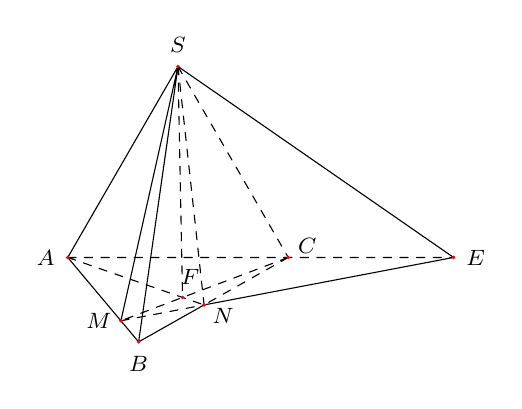
\begin{tikzpicture}[scale=0.7, font=\footnotesize, line join=round, line cap=round, >=stealth]
					\path
					(0,0) coordinate (A)
					(4,0) coordinate (C)
					(-50:2) coordinate (B)
					(60:4) coordinate (S)
					(-50:1.5) coordinate (M)
					(7,0) coordinate (E);
					\coordinate (N) at (intersection cs:first line={(M)--(E)},second line={(C)--(B)});
					\coordinate (F) at (intersection cs:first line={(A)--(N)},second line={(C)--(M)});
					\draw (A)--(B)--(S)--cycle (S)--(M) (B)--(N) (E)--(N) (S)--(E);
					\draw[dashed] (A)--(E) (M)--(N) (C)--(M) (A)--(N) (S)--(F) (S)--(N) (C)--(N) (S)--(C);
					\foreach \x/\g in {A/180,B/-90,C/30,S/90,M/180,N/-30,F/70,E/0}\fill[red] (\x) circle (1pt)+(\g:4mm)node[black]{$\x$};
				\end{tikzpicture}
			}
			\itemch Sai. Trong mặt phẳng $(ABC)$, vẽ giao điểm $F$ của $AN$ và $MC$.\\
			Ta có $S$ và $F$ là hai điểm chung của hai mặt phẳng $(SAN)$ và $(SCM)$.\\
			Suy ra $(SAN)\cap (SCM)=SF$.
	\end{itemchoice}}
\end{ex}


\Closesolutionfile{ans}
\indapan{3}{ans/ans-0-B1-DS}

\Opensolutionfile{ans}[ans/ans-0-B1-KQ]
\caukq


\begin{ex}%[1H4N1-3]
	Cho điểm $S$ nằm ngoài mặt phẳng chứa hình thang $ABCD$, biết $AB\parallel CD$, đáy lớn $AB$, gọi $E=AD\cap BC$. Tìm giao tuyến của hai mặt phẳng $(SBC)$ và $(SAD)$.
	Độ dài giao tuyển cần tìm so với độ dài đoạn $SD$ như thế nào dài hơn chọn $1$, ngắn hơn chọn $2$, bằng nhau chọn $3$, Không so sánh được chọn $4$, không nằm ở trường hợp nào của các lựa chọn trước thì chọn $5$.
	\shortans{$1$}
	\loigiai{
		\immini
		{
			Trong $(ABCD)$, gọi $E=AD\cap BC$.\\
			Ta có $\heva{& E\in AD\subset (SAD) \\ & E\in BC\subset (SBC)} \Rightarrow E\in (SAD)\cap (SBC)$.\\
			Mà $S\in (SAD)\cap (SBC)$\\
			$\Rightarrow SE=(SAD)\cap (SBC)$.
		}
		{
			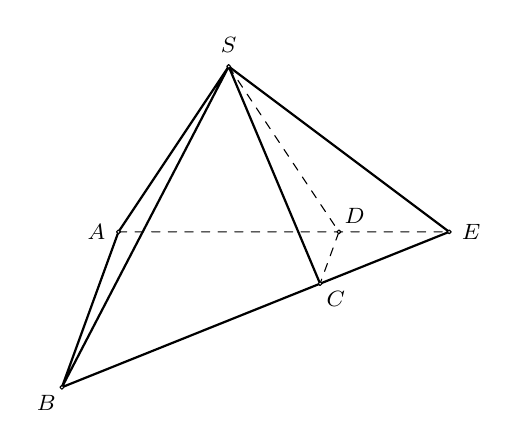
\begin{tikzpicture}[line join = round, line cap = round, >=stealth, font=\footnotesize, scale=0.7]
				\path (0,0)coordinate(A)
				(2,3)coordinate(S)
				(-110:3) coordinate (B)
				(4,0)coordinate(D)
				+(-110:1) coordinate (C)
				(6,0)coordinate(E);
				\draw [dashed] (A)--(E) (S)--(D)--(C);
				\draw [thick](S)--(A)--(B)--(E)--(S)--(C) (S)--(B);
				\foreach \x/\g in {A/180,S/90,C/-45,D/45,B/-135,E/0}\draw[fill=white] (\x) circle (1pt)+(\g:4mm) node{$\x$};
			\end{tikzpicture}
		}
	}
\end{ex}

\begin{ex}%[1H4N1-4]
	Cho tứ diện $ABCD$. Gọi $I$ là trung điểm $AB$, $J$ là điểm thuộc cạnh $AD$ sao cho $JD=\dfrac{1}{3}JA$, gọi $E=IJ\cap BD$. Tìm giao điểm của đường thẳng $IJ$ và mp $(BCD)$. Nếu giao điểm thuộc $(ABD)$ chọn $1$, thuộc $(ACD)$ chọn $2$, thuộc $(ABD)$ chọn $3$, thuộc cạnh $AC$ chọn $4$, không nằm ở trường hợp nào của các lựa chọn trước thì chọn $5$.
	\shortans{$3$}
	\loigiai{
		\immini
		{Trong mặt phẳng $(ABD)$, gọi $ E=IJ\cap BD$.\\
			Ta có $\heva{& E\in IJ \\ & E\in BD\subset (BCD)} \Rightarrow E=IJ\cap (BCD)$.
		}
		{\begin{tikzpicture}[line join = round, line cap = round, >=stealth, font=\footnotesize, scale=0.7]
				\path (0,0)coordinate(B)(2,3)coordinate(A)(-70:2) coordinate (C)
				(4,0)coordinate(D)($(A)!1/2!(B)$)coordinate(I) ($(A)!3/4!(D)$)coordinate(J)
				;
				\coordinate (E) at (intersection cs:first line={(I)--(J)}, second line={(B)--(D)});
				\draw [dashed] (B)--(D) (I)--(J);
				\draw [thick](A)--(B)--(C)--(D)--(E)--(J)--(A)--(C) (J)--(D);
				\foreach \x/\g in {B/180,A/90,C/180,D/-45,J/45,E/0,I/180}\draw[fill=white] (\x) circle (1pt)+(\g:4mm) node{$\x$};
			\end{tikzpicture}
		}
	}
\end{ex}

\begin{ex}%[1H4H1-3]
	Cho hình chóp $S.ABCD$. Gọi $I$ là trung điểm của $SD$, $J$ là điểm trên $SC$ và không trùng trung điểm $SC$, gọi $F=IJ\cap CD$. Tìm giao tuyến của hai mặt phẳng $(ABCD)$ và $(AIJ)$. So sánh chiều dài đoạn giao tuyến cần tìm với $AI$ nếu dài hơn $AI$ chọn $1$, Ngắn hơn $AI$ chọn $2$, Bằng $AI$ chọn $3$, không so sánh được chọn $4$, không nằm ở trường hợp nào của các lựa chọn trước thì chọn $5$.
	\shortans{$1$}
	\loigiai{
		\immini
		{Trong $(ABCD)$ gọi $F=IJ\cap CD$.\\
			Ta có $\heva{& F\in IJ\subset (AIJ)\\ & F\in CD\subset (ABCD)} \Rightarrow F\in (AIJ)\cap (ABCD)$.\\
			Mà $A\in (AIJ)\cap (ABCD)$\\
			$\Rightarrow AF=(ACD)\cap (AEF)$.
		}
		{\begin{tikzpicture}[line join = round, line cap = round, >=stealth, font=\footnotesize, scale=0.7]
				\path (0,0)coordinate(A)(2,3)coordinate(S)(-70:2) coordinate (B)
				(5,0)coordinate(D)+(-120:3) coordinate (C) ($(S)!1/2!(D)$)coordinate(I) ($(S)!3/4!(C)$)coordinate(J)
				;
				\coordinate (F) at (intersection cs:first line={(I)--(J)}, second line={(D)--(C)});
				\coordinate (M) at (intersection cs:first line={(A)--(F)}, second line={(B)--(C)});
				\draw [dashed] (A)--(D) (I)--(A) (A)--(J) (A)--(M) (M)--(C);
				\draw [thick](S)--(A)--(B)--(M)--(F)--(D)--(S)--(C) (S)--(B) (F)--(I);
				\foreach \x/\g in {B/180,A/180,C/-30,D/0,J/0,I/30,S/90,F/-90}\draw[fill=white] (\x) circle (1pt)+(\g:4mm) node{$\x$};
			\end{tikzpicture}
		}
	}
\end{ex}

\begin{ex}%[1H4N1-6]
	Cho ba điểm $A$, $B$, $C$ không thẳng hàng và không thuộc mp $(Q)$, các đường thẳng $BC$, $CA$, $AB$ cắt $(Q)$ lần lượt tại $F$, $E$, $D$. Hỏi ba điểm $D$, $E$, $F$ có thẳng hàng không? có thẳng hàng chọn $1$, không thẳng hàng chọn $2$, trùng nhau chọn $3$, không nằm ở trường hợp nào của các lựa chọn trước thì chọn $4$.
	\shortans{1}
	\loigiai{
		\immini
		{Ta có $F$, $E$, $D$ lần lượt thuộc hai mặt phẳng $(Q)$ và $(ABC)$ nên $F$, $E$, $D$ thuộc giao tuyến $d$ của $(Q)$ và $(ABC)$. \\
			Vậy $D$, $E$, $F$ thẳng hàng.
		}
		{\begin{tikzpicture}[line join = round, line cap = round, >=stealth, font=\footnotesize, scale=0.7]
				\path (0,0)coordinate(M)
				+(-2,-2)coordinate(N)
				+(5,0)coordinate(P)
				($(N)+(P)-(M)$)coordinate(Q) (3,2)coordinate(A) (2,1)coordinate(B) (2.5,0.5)coordinate(C)  (4,-0.5)coordinate(G);
				\coordinate[label=above:$d$] (H)at(-0.9,-1.5);
				\draw pic[angle radius=7mm,draw=blue,fill=green!50,opacity=.5,"$Q$",angle eccentricity=.7] {angle = Q--N--M};
				\coordinate (D) at (intersection cs:first line={(H)--(G)}, second line={(A)--(B)});
				\coordinate (E) at (intersection cs:first line={(H)--(G)}, second line={(A)--(C)});
				\coordinate (F) at (intersection cs:first line={(H)--(G)}, second line={(B)--(C)});
				\draw (H)--(G) (M)--(N)--(Q)--(P)--cycle (A)--(D) (B)--(F) (A)--(E);
				\foreach \x/\g in {B/90,A/0,C/0,D/-90,E/-90,F/-90}\draw[fill=white] (\x) circle (1pt)+(\g:4mm) node{$\x$};
			\end{tikzpicture}
		}
	}
\end{ex}

\begin{ex}%[1H4V4-6]
	Cho hình chóp $S.ABC$. Gọi $M$, $N$ lần lượt là trung điểm của $SA$ và $BC$, $P$ là điểm trên cạnh $AB$ sao cho $\dfrac{AP}{AB}=\dfrac{1}{3}$. Gọi $Q$ là giao điểm của $SC$ với mặt phẳng $(MNP)$. Tính $\dfrac{SC}{SQ}$.
	\shortans{$3$}
	\loigiai{
		\immini
		{Tìm giao điểm $Q$ của $SC$ với mặt phẳng $(MNP)$.\\
			Chọn mặt phẳng phụ $(SAC)$ chứa $SC$.\\
			Trong $(ABC)$ gọi $H=AC\cap NP$.\\
			Suy ra $(MNP)\cap(SAC)=HM$.\\
			Khi đó $Q$ là giao điểm của $HM$ và $SC$.\\
			Gọi $L$ là trung điểm $AC$.
		}
		{\begin{tikzpicture}[scale=0.8, font=\footnotesize, line join=round, line cap=round, >=stealth]
				\path
				(0,0) coordinate (A)
				(3,0) coordinate (C)
				(-50:1.2) coordinate (B)
				(60:4) coordinate (S) ($(S)!1/2!(A)$)coordinate(M) ($(C)!1/2!(B)$)coordinate(N) ($(A)!1/3!(B)$)coordinate(P) ($(C)!1/2!(A)$)coordinate(L);
				\coordinate (H) at (intersection cs:first line={(C)--(A)}, second line={(N)--(P)});
				\coordinate (Q) at (intersection cs:first line={(C)--(S)}, second line={(H)--(M)});
				\draw (S)--(M)--(P)--(B)--(C)--(S)--(B) (H)--(P) (H)--(M);
				\draw[dashed] (M)--(A)--(P) (H)--(C) (P)--(N) (M)--(Q) (M)--(L)--(N)--cycle;
				\foreach \x/\g in {A/120,B/-90,C/0,S/90,H/180,M/110,N/-45,P/-110,Q/0,L/-110}\fill[red] (\x) circle (1pt)+(\g:3mm) node[black]{$\x$};
			\end{tikzpicture}
		}
		\noindent Ta có $\dfrac{HA}{HL}=\dfrac{AP}{LN}=\dfrac{\dfrac{1}{3}AB}{\dfrac{1}{2}AB}=\dfrac{2}{3}$ (vì $M$, $N$ là trung điểm của $AC$ và $BC$ nên $LN=\dfrac{1}{2}AB$).\\
		$\Rightarrow HA=\dfrac{2}{3}HL$.\\
		Mà $LC=AL=HL-HA=HL-\dfrac{2}{3}HL=\dfrac{1}{3}HL$ nên $ HL=\dfrac{3}{4}HC$.\\
		Mặt khác, ta có $\dfrac{HC}{HL}=\dfrac{QC}{ML}=\dfrac{4}{3}$ (vì $ ML\parallel SC$).\\
		Mà $2ML=SC$ nên $\dfrac{QC}{SC}=\dfrac{3}{2}\Rightarrow\dfrac{SC}{SQ}=3$.
	}
\end{ex}

\begin{ex}%[1H4H4-6]
	Cho hình chóp $S.ABCD$ có đáy là hình bình hành. $M$ là trung điểm của $SC$. Gọi $I$ là giao điểm của đường thẳng $AM$ với mặt phẳng $(SBD)$. Tính tỉ số $\dfrac{IA}{IM}$.
	\shortans{$2$}
	\loigiai{
		\immini
		{Gọi $AC\cap BD=O$ thì $(SAC)\cap(SBD)=SO$.\\
			Trong mặt phẳng $(SAC)$, lấy $AM\cap SO=I$\\ $\Rightarrow I=AM\cap(SBD)$.\\
			Do trong $\triangle SAC$, $AM$ và $SO$ là hai đường trung tuyến, nên $I$ là trọng tâm $\triangle SAC$.\\
			Vậy $IA=2IM$.
		}
		{\begin{tikzpicture}[scale=0.7, font=\footnotesize, line join=round, line cap=round, >=stealth]
				\path
				(0,0) coordinate (A)
				(-1.5,-1.5) coordinate (D)
				(4,0) coordinate (B)
				($(B)-(A)+(D)$) coordinate (C)
				($(A)+(0,4)$) coordinate (S) ($(S)!1/2!(C)$)coordinate(M);
				\coordinate (O) at (intersection cs:first line={(C)--(A)}, second line={(B)--(D)});
				\coordinate (I) at (intersection cs:first line={(S)--(O)}, second line={(A)--(M)});
				\draw (S)--(D)--(C)--(B)--cycle (S)--(C)
				;
				\draw[dashed] (A)--(D) (S)--(A)--(B) (A)--(C) (B)--(D) (S)--(O) (A)--(M);
				\foreach \x/\g in {A/180,B/0,C/0,D/180,S/90,O/-90,I/180,M/0}\fill[red] (\x) circle (1pt)+(\g:4mm) node[black]{$ \x $};
			\end{tikzpicture}
		}
		
	}
\end{ex}
\Closesolutionfile{ans}
\indapan{6}{ans/ans-0-B1-KQ}